\documentclass[pdflatex,sn-aps,iicol]{sn-jnl}% American Physical Society (APS) Reference Style
%DIF LATEXDIFF DIFFERENCE FILE
%DIF DEL main.tex      Tue Feb 17 15:50:44 2026
%DIF ADD revised.tex   Tue Mar 17 16:14:49 2026

\usepackage{graphicx}
\usepackage{multirow}
\usepackage{amsmath,amssymb,amsfonts}
\usepackage{amsthm}
\usepackage{mathrsfs}
\usepackage[title]{appendix}
\usepackage{xcolor}
\usepackage{textcomp}
\usepackage{manyfoot}
\usepackage{booktabs}
\usepackage{algorithm}
\usepackage{algorithmicx}
\usepackage{algpseudocode}
\usepackage{listings}

\usepackage{soul}
\usepackage{hyperref}
%DIF 20c20
%DIF < \usepackage{cleveref}
%DIF -------
\usepackage[capitalise]{cleveref} %DIF > 
%DIF -------
\usepackage{microtype}
\hypersetup{colorlinks,
	linkcolor={blue!75!black!80!yellow},
	citecolor={blue!75!black!80!yellow},
	urlcolor={blue!75!black!80!yellow}
}

%DIF 28a28-30
\usepackage{caption} %DIF > 
\captionsetup[figure]{name={Figure}, font=footnotesize, labelfont=bf} %DIF > 
 %DIF > 
%DIF -------
\usepackage{url}
\usepackage[strings]{underscore}
\usepackage{geometry}
\geometry{columnsep=20pt, left=1.5cm, right=1.5cm, top=2cm, bottom=2cm}
\sloppy
 %DIF > 
\setcitestyle{super} %DIF > 
\bibpunct{}{}{,}{s}{,}{,} %DIF > 
 %DIF > 
\crefname{figure}{Figure}{Figures} %DIF > 
\Crefname{figure}{Figure}{Figures} %DIF > 
 %DIF > 
\crefname{equation}{Eq.}{Eqs.} %DIF > 
\Crefname{equation}{Eq.}{Eqs.} %DIF > 
 %DIF > 
\usepackage[utopia]{mathdesign} %DIF > 
\usepackage[OMLmathrm,OMLmathbf]{isomath} %DIF > 
%DIF PREAMBLE EXTENSION ADDED BY LATEXDIFF
%DIF UNDERLINE PREAMBLE %DIF PREAMBLE
\RequirePackage[normalem]{ulem} %DIF PREAMBLE
\RequirePackage{color}\definecolor{RED}{rgb}{1,0,0}\definecolor{BLUE}{rgb}{0,0,1} %DIF PREAMBLE
\providecommand{\DIFaddtex}[1]{{\protect\color{blue}\uwave{#1}}} %DIF PREAMBLE
\providecommand{\DIFdeltex}[1]{{\protect\color{red}\sout{#1}}} %DIF PREAMBLE
%DIF SAFE PREAMBLE %DIF PREAMBLE
\providecommand{\DIFaddbegin}{} %DIF PREAMBLE
\providecommand{\DIFaddend}{} %DIF PREAMBLE
\providecommand{\DIFdelbegin}{} %DIF PREAMBLE
\providecommand{\DIFdelend}{} %DIF PREAMBLE
\providecommand{\DIFmodbegin}{} %DIF PREAMBLE
\providecommand{\DIFmodend}{} %DIF PREAMBLE
%DIF FLOATSAFE PREAMBLE %DIF PREAMBLE
\providecommand{\DIFaddFL}[1]{\DIFadd{#1}} %DIF PREAMBLE
\providecommand{\DIFdelFL}[1]{\DIFdel{#1}} %DIF PREAMBLE
\providecommand{\DIFaddbeginFL}{} %DIF PREAMBLE
\providecommand{\DIFaddendFL}{} %DIF PREAMBLE
\providecommand{\DIFdelbeginFL}{} %DIF PREAMBLE
\providecommand{\DIFdelendFL}{} %DIF PREAMBLE
%DIF HYPERREF PREAMBLE %DIF PREAMBLE
\providecommand{\DIFadd}[1]{\texorpdfstring{\DIFaddtex{#1}}{#1}} %DIF PREAMBLE
\providecommand{\DIFdel}[1]{\texorpdfstring{\DIFdeltex{#1}}{}} %DIF PREAMBLE
\newcommand{\DIFscaledelfig}{0.5}
%DIF HIGHLIGHTGRAPHICS PREAMBLE %DIF PREAMBLE
\RequirePackage{settobox} %DIF PREAMBLE
\RequirePackage{letltxmacro} %DIF PREAMBLE
\newsavebox{\DIFdelgraphicsbox} %DIF PREAMBLE
\newlength{\DIFdelgraphicswidth} %DIF PREAMBLE
\newlength{\DIFdelgraphicsheight} %DIF PREAMBLE
% store original definition of \includegraphics %DIF PREAMBLE
\LetLtxMacro{\DIFOincludegraphics}{\includegraphics} %DIF PREAMBLE
\newcommand{\DIFaddincludegraphics}[2][]{{\color{blue}\fbox{\DIFOincludegraphics[#1]{#2}}}} %DIF PREAMBLE
\newcommand{\DIFdelincludegraphics}[2][]{% %DIF PREAMBLE
\sbox{\DIFdelgraphicsbox}{\DIFOincludegraphics[#1]{#2}}% %DIF PREAMBLE
\settoboxwidth{\DIFdelgraphicswidth}{\DIFdelgraphicsbox} %DIF PREAMBLE
\settoboxtotalheight{\DIFdelgraphicsheight}{\DIFdelgraphicsbox} %DIF PREAMBLE
\scalebox{\DIFscaledelfig}{% %DIF PREAMBLE
\parbox[b]{\DIFdelgraphicswidth}{\usebox{\DIFdelgraphicsbox}\\[-\baselineskip] \rule{\DIFdelgraphicswidth}{0em}}\llap{\resizebox{\DIFdelgraphicswidth}{\DIFdelgraphicsheight}{% %DIF PREAMBLE
\setlength{\unitlength}{\DIFdelgraphicswidth}% %DIF PREAMBLE
\begin{picture}(1,1)% %DIF PREAMBLE
\thicklines\linethickness{2pt} %DIF PREAMBLE
{\color[rgb]{1,0,0}\put(0,0){\framebox(1,1){}}}% %DIF PREAMBLE
{\color[rgb]{1,0,0}\put(0,0){\line( 1,1){1}}}% %DIF PREAMBLE
{\color[rgb]{1,0,0}\put(0,1){\line(1,-1){1}}}% %DIF PREAMBLE
\end{picture}% %DIF PREAMBLE
}\hspace*{3pt}}} %DIF PREAMBLE
} %DIF PREAMBLE
\LetLtxMacro{\DIFOaddbegin}{\DIFaddbegin} %DIF PREAMBLE
\LetLtxMacro{\DIFOaddend}{\DIFaddend} %DIF PREAMBLE
\LetLtxMacro{\DIFOdelbegin}{\DIFdelbegin} %DIF PREAMBLE
\LetLtxMacro{\DIFOdelend}{\DIFdelend} %DIF PREAMBLE
\DeclareRobustCommand{\DIFaddbegin}{\DIFOaddbegin \let\includegraphics\DIFaddincludegraphics} %DIF PREAMBLE
\DeclareRobustCommand{\DIFaddend}{\DIFOaddend \let\includegraphics\DIFOincludegraphics} %DIF PREAMBLE
\DeclareRobustCommand{\DIFdelbegin}{\DIFOdelbegin \let\includegraphics\DIFdelincludegraphics} %DIF PREAMBLE
\DeclareRobustCommand{\DIFdelend}{\DIFOaddend \let\includegraphics\DIFOincludegraphics} %DIF PREAMBLE
\LetLtxMacro{\DIFOaddbeginFL}{\DIFaddbeginFL} %DIF PREAMBLE
\LetLtxMacro{\DIFOaddendFL}{\DIFaddendFL} %DIF PREAMBLE
\LetLtxMacro{\DIFOdelbeginFL}{\DIFdelbeginFL} %DIF PREAMBLE
\LetLtxMacro{\DIFOdelendFL}{\DIFdelendFL} %DIF PREAMBLE
\DeclareRobustCommand{\DIFaddbeginFL}{\DIFOaddbeginFL \let\includegraphics\DIFaddincludegraphics} %DIF PREAMBLE
\DeclareRobustCommand{\DIFaddendFL}{\DIFOaddendFL \let\includegraphics\DIFOincludegraphics} %DIF PREAMBLE
\DeclareRobustCommand{\DIFdelbeginFL}{\DIFOdelbeginFL \let\includegraphics\DIFdelincludegraphics} %DIF PREAMBLE
\DeclareRobustCommand{\DIFdelendFL}{\DIFOaddendFL \let\includegraphics\DIFOincludegraphics} %DIF PREAMBLE
%DIF AMSMATHULEM PREAMBLE %DIF PREAMBLE
\makeatletter %DIF PREAMBLE
\let\sout@orig\sout %DIF PREAMBLE
\renewcommand{\sout}[1]{\ifmmode\text{\sout@orig{\ensuremath{#1}}}\else\sout@orig{#1}\fi} %DIF PREAMBLE
\makeatother %DIF PREAMBLE
%DIF COLORLISTINGS PREAMBLE %DIF PREAMBLE
\RequirePackage{listings} %DIF PREAMBLE
\RequirePackage{color} %DIF PREAMBLE
\lstdefinelanguage{DIFcode}{ %DIF PREAMBLE
%DIF DIFCODE_UNDERLINE %DIF PREAMBLE
  moredelim=[il][\color{red}\sout]{\%DIF\ <\ }, %DIF PREAMBLE
  moredelim=[il][\color{blue}\uwave]{\%DIF\ >\ } %DIF PREAMBLE
} %DIF PREAMBLE
\lstdefinestyle{DIFverbatimstyle}{ %DIF PREAMBLE
	language=DIFcode, %DIF PREAMBLE
	basicstyle=\ttfamily, %DIF PREAMBLE
	columns=fullflexible, %DIF PREAMBLE
	keepspaces=true %DIF PREAMBLE
} %DIF PREAMBLE
\lstnewenvironment{DIFverbatim}{\lstset{style=DIFverbatimstyle}}{} %DIF PREAMBLE
\lstnewenvironment{DIFverbatim*}{\lstset{style=DIFverbatimstyle,showspaces=true}}{} %DIF PREAMBLE
\lstset{extendedchars=\true,inputencoding=utf8}

%DIF END PREAMBLE EXTENSION ADDED BY LATEXDIFF

\begin{document}

\DIFdelbegin %DIFDELCMD < \title[The ABCs of Phase Retrieval]{%%%
\DIFdelend \DIFaddbegin \title[The ABCs of phase retrieval]{\DIFaddend 
The ABCs of \DIFdelbegin \DIFdel{Phase Retrieval}\DIFdelend \DIFaddbegin \DIFadd{phase retrieval}\DIFaddend :
Connecting the \DIFdelbegin \DIFdel{Acronyms }\DIFdelend \DIFaddbegin \DIFadd{acronyms }\DIFaddend of \DIFdelbegin \DIFdel{Scanning Transmission Electron Microscopy
}\DIFdelend \DIFaddbegin \DIFadd{scanning transmission electron microscopy
}\DIFaddend }
\author*[1]{\fnm{Georgios} \sur{Varnavides}} \email{g.varnavides@tudelft.nl}
\author[1]{\fnm{Willem P.M.} \sur{de Kleijne}}
\author[2]{\fnm{Stephanie M.} \sur{Ribet}}

\affil[1]{\orgdiv{Department of Imaging Physics}, \orgname{Delft University of Technology}, \orgaddress{\street{Lorentzweg 1}, \city{Delft}, \postcode{2628 CJ}, \country{The Netherlands}}}
\affil[2]{\orgdiv{National Center for Electron Microscopy, Molecular Foundry}, \orgname{Lawrence Berkeley National Laboratory}, \orgaddress{\street{67 Cyclotron Rd}, \city{Berkeley}, \postcode{CA 94720}, \country{USA}}}

\DIFdelbegin %DIFDELCMD < \abstract{
%DIFDELCMD < High-resolution scanning transmission electron microscopy (STEM) is an indispensable tool for characterizing the structure and properties of materials down to the atomic scale.
%DIFDELCMD < Conventional STEM imaging, however, is limited by the phase problem, whereby the phase of the electron exit wave is lost upon detection.
%DIFDELCMD < Recent advances in diffractive imaging and 4D-STEM have enabled a range of phase retrieval techniques that computationally reconstruct the missing information.
%DIFDELCMD < These approaches offer improved dose efficiency and enhanced  sensitivity to weakly scattering signals, extending quantitative imaging to beam-sensitive materials composed of light elements.
%DIFDELCMD < In this work, we introduce the phase problem in electron microscopy and survey the diverse landscape of phase retrieval techniques used in the field.
%DIFDELCMD < Despite their many acronyms and algorithmic variations, these techniques share a common physical and mathematical foundation.
%DIFDELCMD < We present a unified framework that connects these seemingly distinct methods, from parallax imaging and tilt-corrected bright field (tcBF-STEM), to aberration-corrected bright-field (acBF-STEM), optimum bright field (OBF-STEM) and single-sideband (SSB) ptychography, as well as iterative ptychographic algorithms.
%DIFDELCMD < Based on these insights, we discuss the opportunities and practical limitations of applying these methods across different materials systems, detector designs, and microscope configurations.
%DIFDELCMD < }
%DIFDELCMD < %%%
\DIFdelend \DIFaddbegin \abstract{
High-resolution scanning transmission electron microscopy (S/TEM) is an indispensable tool for characterizing the structure and properties of materials down to the atomic scale.
Conventional S/TEM imaging, however, is limited by the phase problem, whereby the phase of the electron exit wave is lost upon detection.
Recent advances in diffractive imaging and 4D-STEM have enabled a range of phase retrieval techniques that computationally reconstruct the missing information encoded in the phase of the transmission function.
These approaches offer improved dose efficiency and enhanced  sensitivity to weakly scattering signals, extending quantitative imaging to beam-sensitive materials composed of light elements.
In this work, we introduce the phase problem in electron microscopy and survey the diverse landscape of phase retrieval techniques used in the field.
Despite their many acronyms and algorithmic variations, these techniques share a common physical and mathematical foundation.
We present a unified framework that connects these seemingly distinct methods, from parallax imaging and tilt-corrected bright field (tcBF-STEM), to aberration-corrected bright-field (acBF-STEM), optimum bright field (OBF-STEM) and single-sideband (SSB) ptychography, as well as first-moment integrated center of mass techniques (iCOM) and iterative ptychographic algorithms.
Based on these insights, we discuss the opportunities and practical limitations of applying these methods across different materials systems, detector designs, and microscope configurations.
}
\DIFaddend 

\keywords{transmission electron microscopy (TEM); scanning transmission electron microscopy (STEM); nanostructure; crystallographic structure; 2D materials}

\maketitle

\DIFdelbegin \section{\DIFdel{Introduction}}
%DIFAUXCMD
\addtocounter{section}{-1}%DIFAUXCMD
\DIFdelend \DIFaddbegin \begin{figure*}[t]
  \centering
  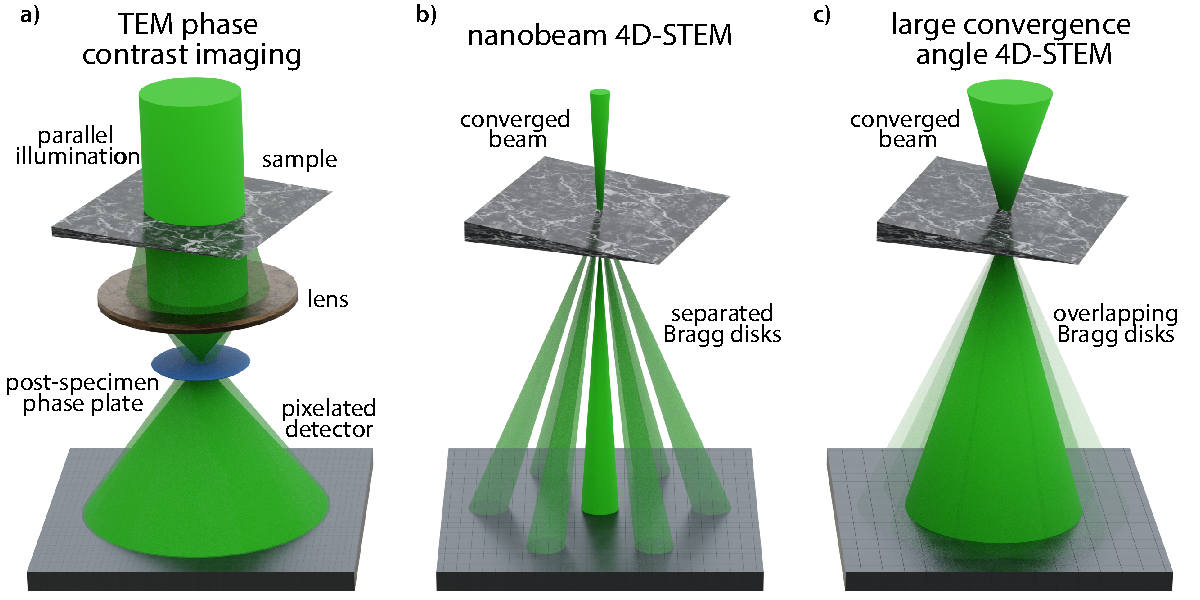
\includegraphics[width=\textwidth]{vector/schematic.pdf}
  \caption{\DIFaddFL{Microscope configurations.
  (a)~TEM Zernike phase-contrast imaging,
  (b)~small-convergence-angle 4D-STEM, used for ``nanobeam'' experiments,
  and (c)~large-convergence-angle 4D-STEM, used for diffractive imaging experiments.}}
  \label{fig:schematic}
\end{figure*}
\DIFaddend 

\DIFaddbegin \section*{\DIFadd{Introduction}}

\DIFaddend Scanning transmission electron microscopy (S/TEM) enables the characterization of specimens from the micron scale down to the atomic scale, making it an indispensable characterization tool for any materials scientist~\cite{Williams_2009}.
S/TEM instruments operate in two complimentary acquisition modalities: \emph{imaging mode}, which produces a magnified real-space image of the specimen, and \emph{diffraction mode}, which records the angular distribution of scattered electrons in reciprocal space~\cite{Carter_2016}.

Traditional parallel-illumination TEM imaging is widely used across disciplines, from high-resolution studies of frozen-hydrated biomolecules~\cite{Vinothkumar_2016} to lattice-resolved~\cite{Alcorn_2023} and defect~\cite{Fultz_2013} imaging of materials.
In contrast, STEM employs a highly converged electron probe containing a broad range of incident wavevectors. 
When this probe interacts with the specimen, it produces a diffraction pattern that encodes the local scattering. 
In this sense, STEM is inherently a diffraction-mode technique, although real-space images can be obtained by processing the resulting position-resolved diffraction patterns -- a process we will refer to as \emph{diffractive imaging}.
This approach routinely provides interpretable \DIFdelbegin \DIFdel{, atomic-resolution imaging of crystalline materials }\DIFdelend \DIFaddbegin \DIFadd{images of materials down to atomic resolution }\DIFaddend and forms the basis of modern \DIFdelbegin \DIFdel{materials }\DIFdelend \DIFaddbegin \DIFadd{crystallographic }\DIFaddend characterization~\cite{Ophus_2023}.

Both \DIFaddbegin \DIFadd{TEM and STEM }\DIFaddend modalities are fundamentally limited by the microscopy ``phase problem,'' first recognized in quantum scattering by Max Born~\cite{born1926quantenmechanik} and discussed in his Nobel Lecture~\cite{born1954}.
Here, we focus on the mathematical foundations of STEM phase-retrieval techniques, which reconstruct the missing phase and thereby overcome these intrinsic contrast limitations.
We emphasize the implications of these methods for quantitative materials characterization and set the stage for a unified treatment of the underlying physics.

\DIFdelbegin %DIFDELCMD < \begin{figure*}[t]
%DIFDELCMD <   \centering
%DIFDELCMD <   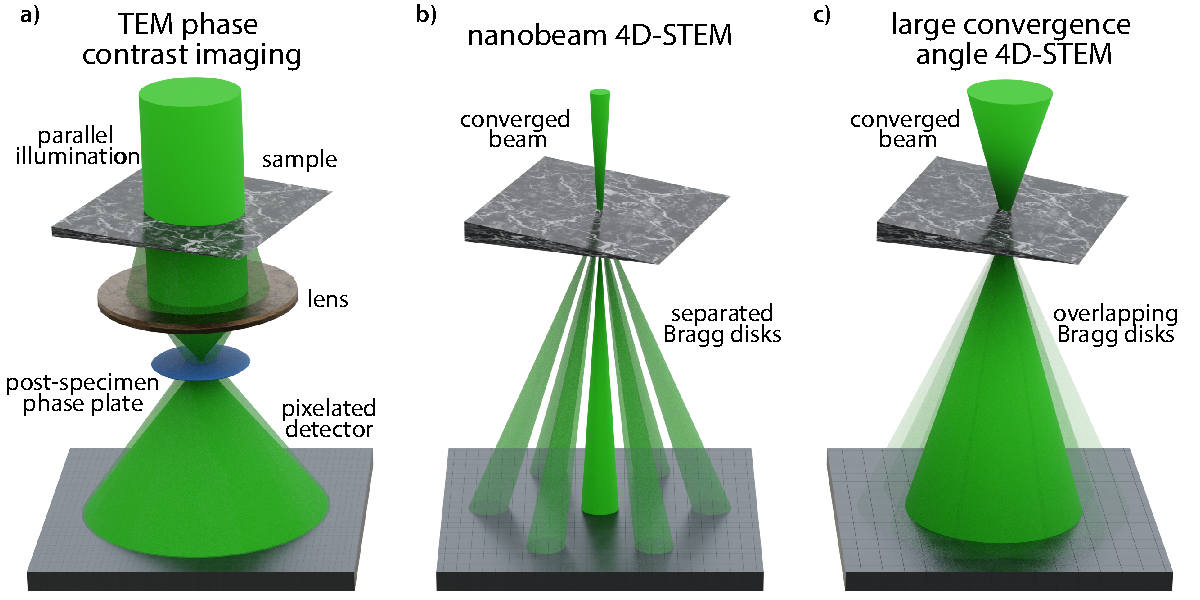
\includegraphics[width=\textwidth]{vector/schematic.pdf}
%DIFDELCMD <   %%%
%DIFDELCMD < \caption{%
{%DIFAUXCMD
\DIFdelFL{Microscope configurations.
  (a)~TEM Zernike phase-contrast imaging,
  (b)~small-convergence-angle 4D-STEM, used for ``nanobeam'' experiments,
  and (c)~large-convergence-angle 4D-STEM, used for diffractive imaging experiments.}}
  %DIFAUXCMD
%DIFDELCMD < \label{fig:schematic}
%DIFDELCMD < \end{figure*}
%DIFDELCMD < %%%
\DIFdelend \DIFaddbegin \DIFadd{The phase problem also has direct practical consequences for real-world experiments.
In biological imaging, phase contrast is essential for visualizing proteins~\mbox{%DIFAUXCMD
\cite{Berk_2024,Yu_2025,Spoth_2017}}\hskip0pt%DIFAUXCMD
.
In materials science, it enables the detection of low atomic number species, such as lithium and oxygen in functional and quantum materials~\mbox{%DIFAUXCMD
\cite{lozano2018low,kp2025electron}}\hskip0pt%DIFAUXCMD
, and the characterization of beam-sensitive systems, including metal–organic frameworks~\mbox{%DIFAUXCMD
\cite{shen2020imaging, Li_2025, Ma_2025}}\hskip0pt%DIFAUXCMD
.
These challenges arise across a wide range of specimen classes, including nanoparticles~\mbox{%DIFAUXCMD
\cite{shi2025electron,Ribet_2024,Varnavides_2023}}\hskip0pt%DIFAUXCMD
, one-dimensional nanostructures such as nanotubes~\mbox{%DIFAUXCMD
\cite{yang2016simultaneous,pelz2023solving}}\hskip0pt%DIFAUXCMD
, two-dimensional materials~\mbox{%DIFAUXCMD
\cite{jiang2018electron,o2022increasing,Susi_2025,byrne2025fabrication,zhang2025atom}}\hskip0pt%DIFAUXCMD
, thin films~\mbox{%DIFAUXCMD
\cite{dong2025sub}}\hskip0pt%DIFAUXCMD
, and cross-sectional views of thicker crystalline samples~\mbox{%DIFAUXCMD
\cite{scheid2025atomic,chen2024imaging}}\hskip0pt%DIFAUXCMD
.
Realizing these capabilities in practice requires both high-quality data acquisition and robust reconstruction strategies.
Motivated by this, we present a unified, mathematically grounded overview of diffractive imaging methods, highlighting their respective strengths and limitations.
}\DIFaddend 

\DIFdelbegin \subsection{\DIFdel{Microscopy Phase Problem}}
%DIFAUXCMD
\addtocounter{subsection}{-1}%DIFAUXCMD
\DIFdelend \DIFaddbegin \subsection*{\DIFadd{Microscopy phase problem}}
\DIFaddend 

The phase problem arises in electron microscopy because the scattered electron wavefunction -- the ``exit wave'' -- is complex-valued, yet physical detectors only measure real-valued intensities~\cite{Fienup_1982}.
In other words, although the specimen primarily imprints a \emph{phase shift} on the complex incident electron wavefunction $\psi$, the detector records $|\psi|^2$, seemingly discarding the information that carries most of the specimen's structure~\cite{born1954}.

For S/TEM, this becomes clear in the wave propagation formalism.
The evolution of an electron wavefunction, $\psi(\boldsymbol{r})$, along the optical axis $z$ is governed by the Schr\"odinger equation for fast electrons~\cite{Kirkland_2020}:
\begin{equation}
  \frac{\partial \psi(\boldsymbol{r})}{\partial z} = \frac{i \lambda}{4\pi}\nabla_{xy}^2 \psi(\boldsymbol{r})
  + i \sigma V(\boldsymbol{r}) \psi(\boldsymbol{r}),
  \label{eq:schrodinger}
\end{equation}
where $\lambda$ is the relativistic wavelength, $\sigma$ the interaction constant, $\nabla_{xy}^2$ the in-plane Laplacian operator, and $V(\boldsymbol{r})$ the specimen electrostatic potential.

The two terms on the right-hand side of \cref{eq:schrodinger} are the propagation and transmission operators.
Because these operators do not commute, numerical solutions typically use a split-step algorithm known as the multislice method~\cite{Cowley_1957}.
The specimen is partitioned into $n$ thin slices, and the wavefunction is updated by alternating between transmission through each slice and free-space propagation~\cite{Kirkland_2020}:
\begin{align}
  \psi_{n+1}(\boldsymbol{r}) &= \exp\!\left[\frac{i \lambda \Delta z}{4\pi}\nabla_{xy}^2\right]
  \exp\!\left[i \sigma V_n^{\Delta z}(\boldsymbol{r})\right] \psi_n(\boldsymbol{r}),
  \label{eq:ms} \\
  V_n^{\Delta z}(\boldsymbol{r}) &= \int_{z_n}^{z_n+\Delta z} V(\boldsymbol{r})\,\mathrm{d}z.
  \label{eq:projected-pot}
\end{align}
Inspecting \cref{eq:ms,eq:projected-pot} shows that the specimen information enters solely through a multiplicative phase factor $\exp\!\left[i \sigma V_n^{\Delta z}(\boldsymbol{r})\right]$.
Electrons are not absorbed by the specimen (ignoring weak inelastic losses), and any apparent amplitude modulation simply reflects electrons scattered outside the acceptance angle of the detector.
Thus, the structural information of interest to materials scientists is encoded in the phase of the exit wave, not its magnitude.
Recovering the exit-wave phase from intensity-only measurements is therefore the central challenge.

\begin{figure*}[t]
  \centering
  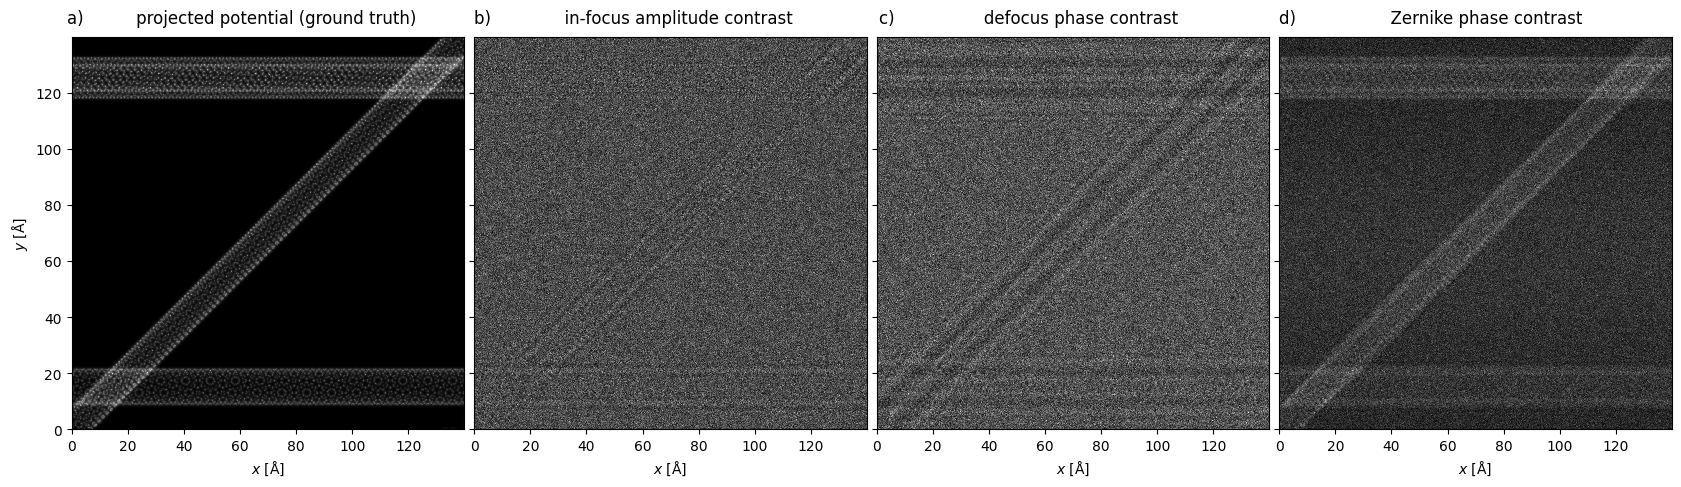
\includegraphics[width=\textwidth]{raster/phase_contrast_imaging_CNTs.png}
  \caption{Simulated high-resolution TEM imaging
  (a)~of single- and double-walled carbon nanotubes, acquired with an electron dose \DIFdelbeginFL \DIFdelFL{ofv}\DIFdelendFL \DIFaddbeginFL \DIFaddFL{of }\DIFaddendFL $500~\mathrm{e}/\text{\AA}^2$ using:
  (b)~in-focus optics,
  (c)~$50$~nm of over-focus,
  and (d)~an ideal Zernike phase plate.}
  \label{fig:pci}
\end{figure*}

\DIFdelbegin \subsection{\DIFdel{Phase Contrast Imaging}}
%DIFAUXCMD
\addtocounter{subsection}{-1}%DIFAUXCMD
\DIFdelend \DIFaddbegin \subsection*{\DIFadd{Phase contrast imaging}}
\DIFaddend 

A direct approach to the microscopy phase problem is to leverage the imaging optics to convert otherwise imperceptible phase variations in the exit wave into measurable intensity variations in the imaging plane.
This approach, known as \emph{phase contrast imaging} (PCI)~\cite{Carter_2016}, is most naturally implemented in plane-wave TEM, where the objective lens forms a magnified real-space image of the specimen.

To illustrate the basic principle, we restrict our attention to weakly-scattering specimens satisfying the \emph{weak phase object approximation} (WPOA), for which the exit wave can be written as~\cite{Vulovic_2014}
\begin{equation}
  \psi_{\text{exit}}(\boldsymbol{r}) \approx 1 + i \sigma V_p(\boldsymbol{r}) + \mathcal{O}\!\left(\sigma^2 V_p^2(\boldsymbol{r})\right),
  \label{eq:wpoa}
\end{equation}
where $V_p(\boldsymbol{r}) = \int_{-\infty}^{\infty} V(\boldsymbol{r})\,\mathrm{d}z$ is the projected sample potential and terms quadratic in the interaction constant are neglected.
In this regime the specimen modifies only the phase of the electron wavefunction, so optical manipulations are required to convert the phase into measurable amplitude contrast.

\DIFdelbegin \subsubsection{\DIFdel{Defocus Phase Contrast}}
%DIFAUXCMD
\addtocounter{subsubsection}{-1}%DIFAUXCMD
\DIFdelend \DIFaddbegin \subsubsection*{\DIFadd{Defocus phase contrast}}
\DIFaddend 

The simplest such manipulation is intentional over- or under-focus of the objective lens.
Defocus by a value $\Delta f$ multiplies the exit wave in reciprocal space by a quadratic phase factor given by
\begin{equation}
  \tilde{\psi}'(\boldsymbol{q}) = \exp\!\left[-i \pi \lambda \Delta f \lvert \boldsymbol{q} \rvert^2 \right] \tilde{\psi}(\boldsymbol{q}).
  \label{eq:defocus}
\end{equation}
Transforming this to real space and expanding to first order in $\sigma V_p(\boldsymbol{r})$, the image intensity becomes
\begin{equation}
  I(\boldsymbol{r}) \approx 1 - 2\sigma \bigl[ V_p(\boldsymbol{r}) \circledast h_{\Delta f}(\boldsymbol{r}) \bigr],
  \label{eq:defocus-int}
\end{equation}
where $h_{\Delta f}(\boldsymbol{r}) = \mathcal{F}^{-1}_{\boldsymbol{q}\rightarrow\boldsymbol{r}} \!\left\{ \sin\!\left[\pi \lambda \Delta f \lvert \boldsymbol{q} \rvert^2 \right] \right\}$ is the real-space convolution kernel corresponding to \cref{eq:defocus}, and $\circledast$ represents the convolution operation.
Defocus thus converts sample-induced phase variations into intensity contrast through a sinusoidal convolution, leading to characteristic contrast reversals with increasing spatial frequency.

\DIFdelbegin \subsubsection{\DIFdel{Phase Plate Contrast}}
%DIFAUXCMD
\addtocounter{subsubsection}{-1}%DIFAUXCMD
\DIFdelend \DIFaddbegin \subsubsection*{\DIFadd{Phase plate contrast}}
\DIFaddend 

Another approach is to introduce a phase shift using a post-specimen phase plate (\cref{fig:schematic}a).
Originating from optical phase-contrast microscopy, this technique was awarded the 1953 Nobel Prize in Physics for its transformative impact on biological imaging~\cite{Zernike_1942}.
An ideal phase plate shifts the unscattered beam by $\pi/2$:
\begin{equation}
  \tilde{\psi}'(\boldsymbol{q}) = \begin{cases} i\,\tilde{\psi}(\boldsymbol{q}), & \text{if } \boldsymbol{q}=\boldsymbol{0}, \\ \tilde{\psi}(\boldsymbol{q}), & \text{otherwise}. \end{cases}
  \label{eq:zernike}
\end{equation}
Expanding again to first order in $\sigma V_p(\boldsymbol{r})$, the corresponding image intensity is given by
\begin{equation}
  I(\boldsymbol{r}) \approx 1 + 2\sigma V_p(\boldsymbol{r}),
  \label{eq:zernike-int}
\end{equation}
showing that a phase plate enables direct, linear transfer of the specimen phase into image intensity.

\Cref{fig:pci} illustrates these effects for a simulated three-dimensional arrangement of single- and double-walled carbon nanotubes (CNTs) \DIFdelbegin \DIFdel{acquired at low dose.
The }\DIFdelend \DIFaddbegin \DIFadd{under low-dose conditions.
The projected potential is shown in \mbox{%DIFAUXCMD
\cref{fig:pci}}\hskip0pt%DIFAUXCMD
a.
The }\DIFaddend in-focus HRTEM image \DIFdelbegin \DIFdel{shows almost no contrast, especially for the top nanotube , which is exactly }\DIFdelend \DIFaddbegin \DIFadd{(\mbox{%DIFAUXCMD
\cref{fig:pci}}\hskip0pt%DIFAUXCMD
b) exhibits minimal contrast, particularly for the nanotube located }\DIFaddend at the focal plane\DIFdelbegin \DIFdel{of the microscope.
Defocus improves visibility but introduces }\DIFdelend \DIFaddbegin \DIFadd{, directly reflecting the phase problem.
Introducing defocus (\mbox{%DIFAUXCMD
\cref{fig:pci}}\hskip0pt%DIFAUXCMD
c) enhances visibility but induces }\DIFaddend frequency-dependent contrast reversals, causing different regions of the CNTs to appear \DIFdelbegin \DIFdel{in or }\DIFdelend \DIFaddbegin \DIFadd{alternately in and }\DIFaddend out of focus.
\DIFaddbegin \DIFadd{In contrast, }\DIFaddend Zernike phase contrast \DIFdelbegin \DIFdel{recovers both the }\DIFdelend \DIFaddbegin \DIFadd{(\mbox{%DIFAUXCMD
\cref{fig:pci}}\hskip0pt%DIFAUXCMD
d) restores both }\DIFaddend high-resolution lattice \DIFdelbegin \DIFdel{information }\DIFdelend \DIFaddbegin \DIFadd{detail }\DIFaddend and the low-frequency envelope\DIFdelbegin \DIFdel{distinguishing }\DIFdelend \DIFaddbegin \DIFadd{, enabling clear discrimination of }\DIFaddend the CNTs from vacuum.

\DIFdelbegin \subsection{\DIFdel{Diffractive Imaging}}
%DIFAUXCMD
\addtocounter{subsection}{-1}%DIFAUXCMD
\DIFdelend \DIFaddbegin \subsection*{\DIFadd{Diffractive imaging}}
\DIFaddend 

As discussed above, STEM is inherently a diffraction-based technique: at each probe position $\boldsymbol{R}$, we have access to the diffraction intensity $I(\boldsymbol{R},\boldsymbol{k}) = \lvert \tilde{\psi}_{\text{exit}}(\boldsymbol{R},\boldsymbol{k}) \rvert^2$, where $\boldsymbol{k}$ is the in-plane scattering vector.
Historically, STEM has used monolithic annular detectors that integrate this intensity within annular collection limits to form a real-space image.
A conventional annular signal is therefore given by
\begin{equation}
  I_{\text{ann}}(\boldsymbol{R}) = \int_{\theta_{\text{in}}}^{\theta_{\text{out}}} I(\boldsymbol{R},\boldsymbol{k})\,\mathrm{d}\boldsymbol{k},
  \label{eq:annular-int}
\end{equation}
yielding familiar contrast modes such as bright-field (BF), annular bright-field (ABF), annular dark-field (ADF), and high-angle annular dark-field (HAADF) STEM~\cite{Crewe_1970,Pennycook_1991}.
Dark-field images in particular are highly interpretable \DIFdelbegin \DIFdel{-- especially for crystalline specimens -- }\DIFdelend leading to their prevalence in materials science characterization~\cite{Ophus_2023}.
However, they discard sensitive information encoded in the exit-wave phase and are often not sufficiently electron-dose efficient for beam-sensitive samples.

The development of fast, low-noise direct-electron detectors~\cite{Levin_2021} has enabled recording the full diffraction pattern $I(\boldsymbol{R},\boldsymbol{k})$ at every scan position, giving rise to a family of techniques collectively known as 4D-STEM~\cite{Ophus_2019}.
These datasets retain the full diffractive signature of the probe–specimen interaction, far beyond what can be accessed with scalar annular signals.
Small convergence-angle (``nanobeam'') and large convergence-angle (diffractive imaging) geometries are shown in \cref{fig:schematic}b-c, respectively.
In this review, we focus on the large class of approaches that computationally recover the phase of the specimen from this set of diffraction patterns, which relies on a large convergence angle (\cref{fig:schematic}c).
We refer to this class of approaches as diffractive imaging or STEM \emph{phase-retrieval} techniques~\cite{sanchez2025}.

\begin{figure*}[t]
  \centering
  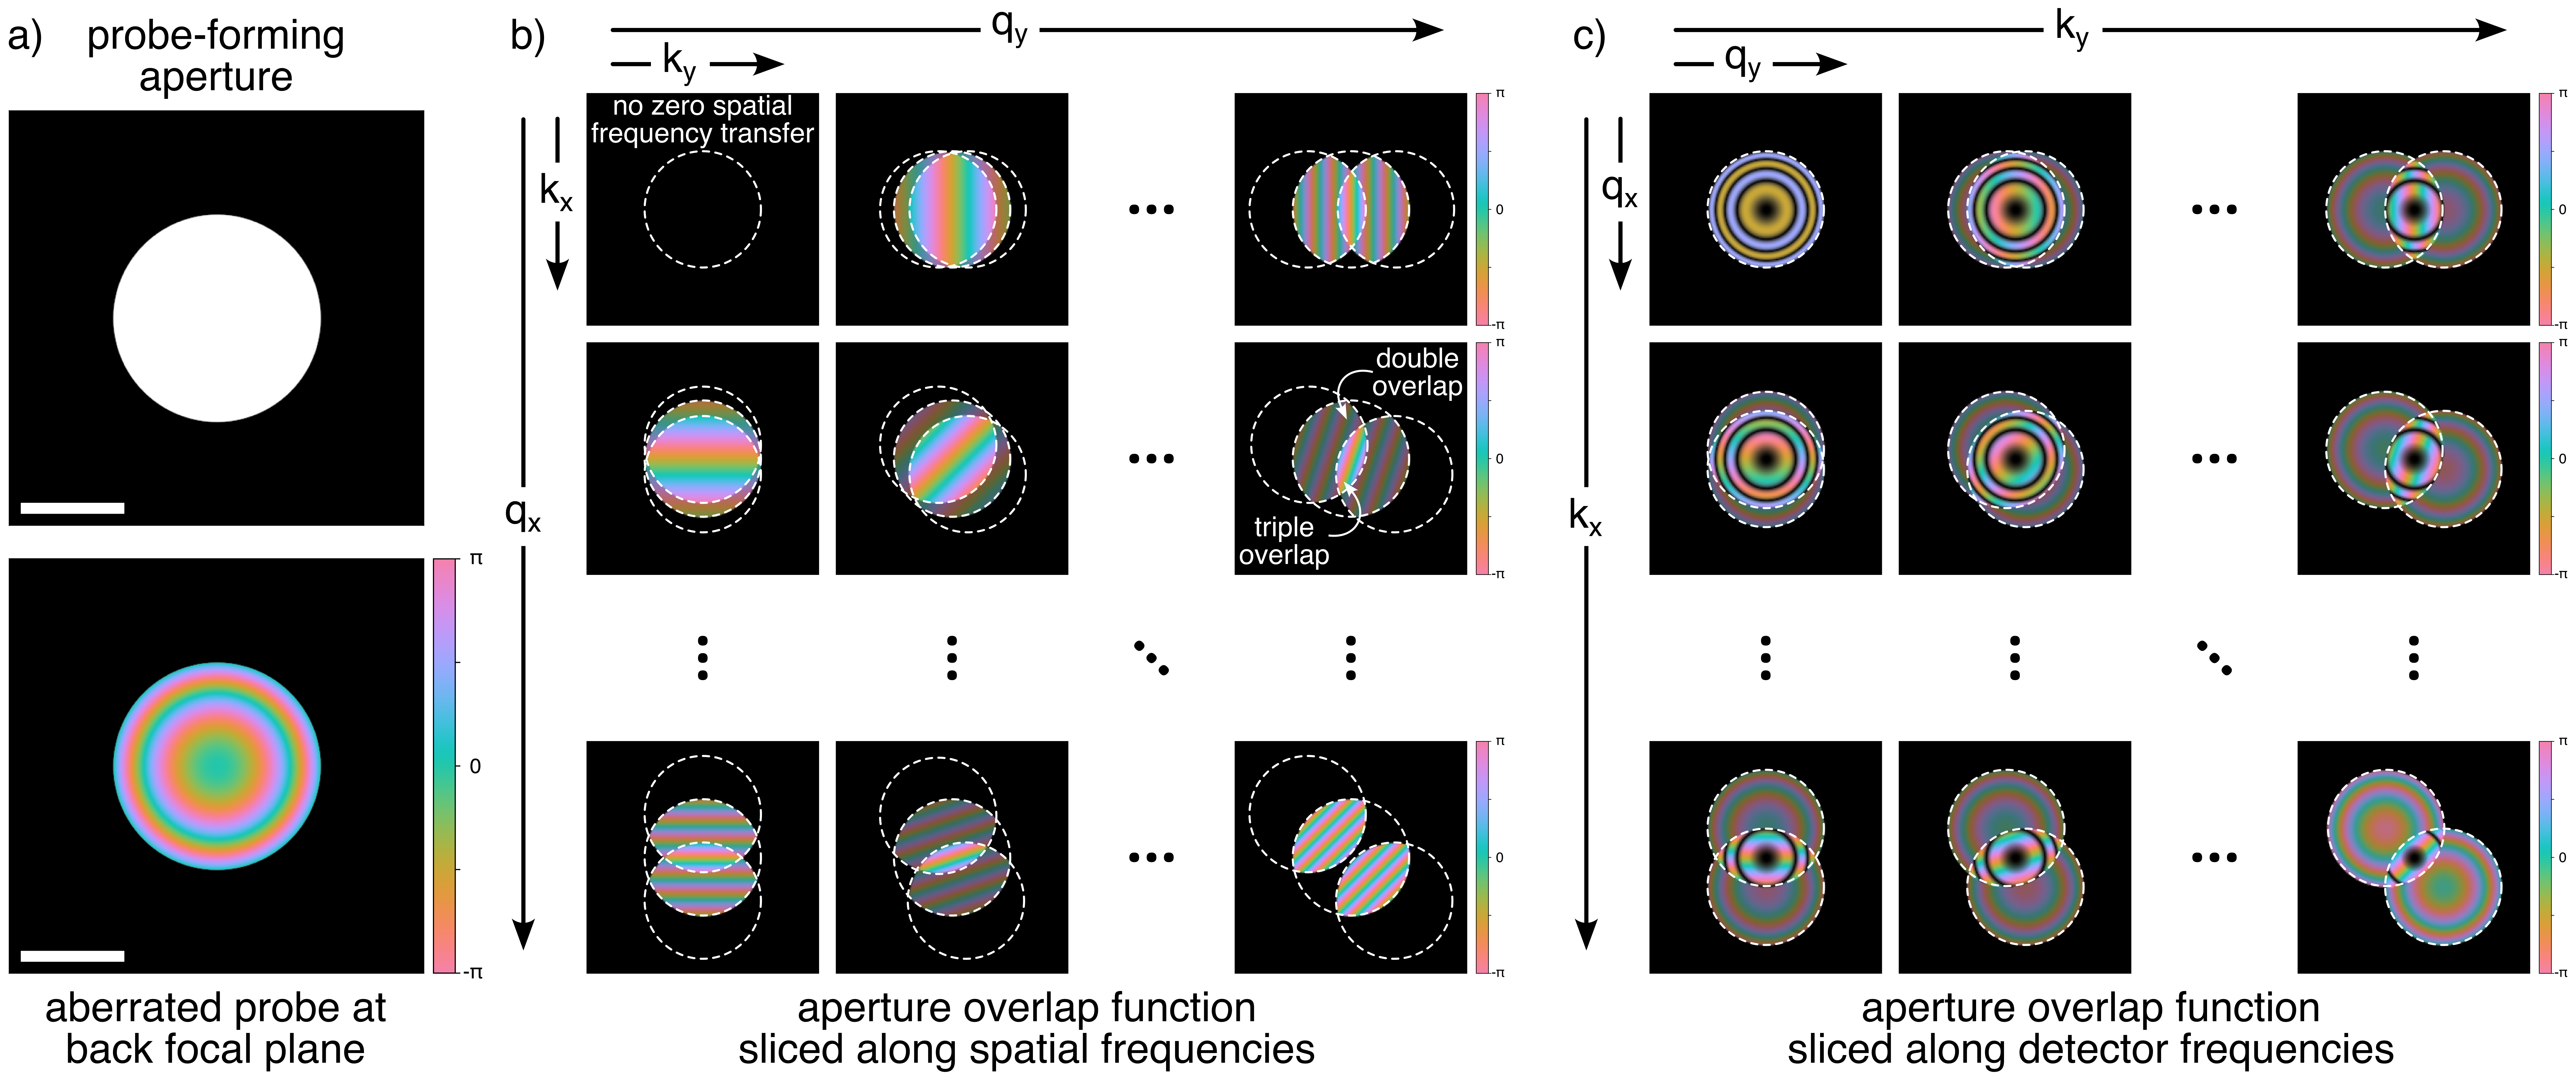
\includegraphics[width=\textwidth]{raster/mrs-bulletin-fig2.png}
  \caption{Components of the aperture overlap function, $\Gamma(\boldsymbol{q},\boldsymbol{k})$.
  (a)~Probe-forming aperture with (bottom) and without (top) aberration function at the back focal plane.
  (b)~Slices along spatial frequencies $\boldsymbol{q}$ plotted over detector frequencies $\boldsymbol{k}$, highlighting the so-called ``double'' and ``triple'' overlap (``trotter'') regions.
  (c)~Slices along detector frequencies $\boldsymbol{k}$ plotted over spatial frequencies $\boldsymbol{q}$, illustrating the effect of shifting the probe aperture and aberrations.}
  \label{fig:gamma}
\end{figure*}

\DIFdelbegin \subsubsection{\DIFdel{Weak Phase Object Approximation}}
%DIFAUXCMD
\addtocounter{subsubsection}{-1}%DIFAUXCMD
\DIFdelend \DIFaddbegin \subsubsection*{\DIFadd{Weak phase object approximation}}
\DIFaddend 

Under the WPOA in \cref{eq:wpoa}, the specimen transmission function is $t(\boldsymbol{r}) \approx 1 + i \sigma V_p(\boldsymbol{r})$, with the Fourier transform of the scattered component given by \DIFdelbegin \DIFdel{$\tilde{\phi}(\boldsymbol{k}) = \mathcal{F}_{\boldsymbol{r}\rightarrow\boldsymbol{k}}\{t(\boldsymbol{r})\}$}\DIFdelend \DIFaddbegin \DIFadd{$\tilde{\phi}(\boldsymbol{k}) = \mathcal{F}_{\boldsymbol{r}\rightarrow\boldsymbol{k}}\{\sigma V_p(\boldsymbol{r})\}$}\DIFaddend .
In this regime, the diffraction intensity can be written as the self-convolution of the converged probe $\tilde{\psi}(\boldsymbol{k})$ with the \DIFdelbegin \DIFdel{WPOA }\DIFdelend \DIFaddbegin \DIFadd{Fourier transform of the transmission function $\tilde{t}(\boldsymbol{k}) = \delta(\boldsymbol{k}) + i \tilde{\phi}(\boldsymbol{k})$ }\DIFaddend term~\cite{Rodenburg_1993}:
\begin{align}
  I(\boldsymbol{R},\boldsymbol{k}) = \iint\, &\tilde{\psi}(\boldsymbol{k}')
  \DIFdelbegin %DIFDELCMD < \tilde{\phi}%%%
\DIFdelend \DIFaddbegin \tilde{t}\DIFaddend (\boldsymbol{k}-\boldsymbol{k}')
  \tilde{\psi}^{*}(\boldsymbol{k}'')
  \DIFdelbegin %DIFDELCMD < \tilde{\phi}%%%
\DIFdelend \DIFaddbegin \tilde{t}\DIFaddend ^{*}(\boldsymbol{k}-\boldsymbol{k}'') \nonumber \\
  &\times \exp\!\left[2\pi i\,\boldsymbol{R}\cdot(\boldsymbol{k}'-\boldsymbol{k}'')\right]
  \,\mathrm{d}\boldsymbol{k}'\,\mathrm{d}\boldsymbol{k}'' .
  \label{eq:wpoa-intensity}
\end{align}

Following Rodenburg et al.~\cite{Rodenburg_1993}, it is convenient to take the Fourier transform of the measured intensities with respect to the scan position, $G(\boldsymbol{q},\boldsymbol{k}) = \mathcal{F}_{\boldsymbol{R}\rightarrow\boldsymbol{q}}\{I(\boldsymbol{R},\boldsymbol{k})\}$, where $\boldsymbol{q}$ is the reciprocal variable corresponding to the \DIFdelbegin \DIFdel{real-space coordinate $\boldsymbol{r}$}\DIFdelend \DIFaddbegin \DIFadd{scan coordinate $\boldsymbol{R}$}\DIFaddend .
Using the identity \DIFdelbegin \DIFdel{$\tilde{\phi}(\boldsymbol{k}) = -\tilde{\phi}^{*}(-\boldsymbol{k})$}\DIFdelend \DIFaddbegin \DIFadd{$\tilde{\phi}(\boldsymbol{k}) = \tilde{\phi}^{*}(-\boldsymbol{k})$}\DIFaddend ~\cite{Rodenburg_1993}, one obtains~\cite{Yang_2016}
\begin{align}
  G(\boldsymbol{q},\boldsymbol{k}) &= \lvert \tilde{\psi}(\boldsymbol{k}) \rvert^2 \delta(\boldsymbol{q}) + \Gamma(\boldsymbol{q},\boldsymbol{k})\,\tilde{\phi}(\boldsymbol{q}), \\
  \Gamma(\boldsymbol{q},\boldsymbol{k}) &\equiv \tilde{\psi}^{*}(\boldsymbol{k})\tilde{\psi}(\boldsymbol{k}-\boldsymbol{q}) - \tilde{\psi}(\boldsymbol{k})\tilde{\psi}^{*}(\boldsymbol{k}+\boldsymbol{q}),
  \label{eq:wpoa-forward}
\end{align}
where the aperture overlap function $\Gamma(\boldsymbol{q},\boldsymbol{k})$ encapsulates the probe geometry and forms the basis of all non-iterative STEM phase-retrieval methods.
\cref{fig:gamma} shows characteristic views of $\Gamma(\boldsymbol{q},\boldsymbol{k})$ for a defocused probe with a circular aperture.

We take the probe to have the form $\tilde{\psi}(\boldsymbol{k}) = A(\boldsymbol{k})\,\exp[-i\chi(\boldsymbol{k})]$, where $A(\boldsymbol{k})$ is a top-hat function describing the probe-forming aperture and $\chi(\boldsymbol{k})$ is the aberration surface given by
\begin{equation}
  \chi(\boldsymbol{k}) = \frac{2\pi}{\lambda} \sum_{n,m} \frac{1}{n+1} C_{n,m} (k\lambda)^{n+1} \cos\!\left[m(\theta-\theta_{n,m})\right],
  \label{eq:chi}
\end{equation}
with $k=\lvert\boldsymbol{k}\rvert$, $\theta=\arctan(\boldsymbol{k})$, and $n$ and $m$ the radial and azimuthal orders of the aberration coefficients $C_{n,m}$ with axes $\theta_{n,m}$.

\DIFdelbegin \subsubsection{\DIFdel{Transfer of Information}}
%DIFAUXCMD
\addtocounter{subsubsection}{-1}%DIFAUXCMD
\DIFdelend \DIFaddbegin \subsubsection*{\DIFadd{Transfer of information}}
\DIFaddend 

Under the WPOA, STEM image formation is linear in the specimen phase.
This allows us to define a contrast transfer function, $\mathrm{CTF}(\boldsymbol{q})$, describing how well spatial frequencies of the specimen are transmitted or, in the context of STEM phase-retrieval techniques, how faithfully they can be reconstructed.
We write the reconstructed phase as
\begin{equation}
  \tilde{\psi}_{\text{rec}}(\boldsymbol{q}) = 2\,\tilde{\phi}(\boldsymbol{q})\,\mathrm{CTF}(\boldsymbol{q}),
  \label{eq:recon-ctf}
\end{equation}
where the factor of $2$ follows common conventions~\cite{Dwyer_2024,Vega_2025}.
An ideal phase-retrieval method would therefore satisfy $\mathrm{CTF}_{\text{ideal}}(\boldsymbol{q})=1$.

For an arbitrary detector response function $D_j(\boldsymbol{k})$ (with $j$ indexing a detector pixel or segment), Hammel and Rose~\cite{Hammel_1995} showed that the complex-valued CTF is~\cite{Hammel_1995,rose_1977}
\begin{align}
  \mathrm{CTF}_j(\boldsymbol{q}) = \frac{i}{2} \int
    &D_j(\boldsymbol{k})\,\tilde{\psi}^{*}(\boldsymbol{k})\tilde{\psi}(\boldsymbol{q}-\boldsymbol{k}) \nonumber \\
    - &D_j(\boldsymbol{k})\,\tilde{\psi}(\boldsymbol{k})\tilde{\psi}^{*}(\boldsymbol{q}+\boldsymbol{k})
  \,\mathrm{d}\boldsymbol{k}.
  \label{eq:ctf}
\end{align}

For a pixelated detector, \DIFdelbegin \DIFdel{$D_j(\boldsymbol{k})=\delta(\boldsymbol{k})$}\DIFdelend \DIFaddbegin \DIFadd{$D_j(\boldsymbol{k})=\delta(\boldsymbol{k}-\boldsymbol{k}_j)$}\footnote{\DIFadd{Note that, for notational convenience, in what follows we simply use $\boldsymbol{k}$ instead of $\boldsymbol{k}_j$ for the detector pixel coordinate.}}\DIFaddend , the integrand reduces to the aperture-overlap function $\Gamma(\boldsymbol{q},\boldsymbol{k})$.
More compact expressions follow from an asymmetric decomposition of cross-correlations~\cite{Bekkevold_2025,Lazic_2017}:
\begin{align}
  \Re\{\mathrm{CTF}_j(\boldsymbol{q})\} &= \frac{1}{2}
   \Big(
    [\psi \star (\psi D_j)](\boldsymbol{q})
    \DIFdelbegin \DIFdel{+
    }\DIFdelend \DIFaddbegin \DIFadd{-
    }\DIFaddend [(\psi D_j)\star \psi](\boldsymbol{q})
  \Big),
  \label{eq:ctf-corr-real} \\
  \Im\{\mathrm{CTF}_j(\boldsymbol{q})\} &= \frac{1}{2}
  \Big(
    [\psi \star (\psi D_j)](\boldsymbol{q})
    \DIFdelbegin \DIFdel{- }\DIFdelend \DIFaddbegin \DIFadd{+
    }\DIFaddend [(\psi D_j)\star \psi](\boldsymbol{q})
  \Big),
  \label{eq:ctf-corr-imag}
\end{align}
where $\star$ denotes cross-correlation and $\Re\{\cdot\}$ and $\Im\{\cdot\}$ represent real and imaginary components.

Two limiting cases of \cref{eq:ctf} provide further physical insight.
In the absence of aberrations, $\chi(\boldsymbol{k})=0$, \DIFdelbegin \DIFdel{the }\DIFdelend \DIFaddbegin \DIFadd{and summing over all detector pixels $D_j$ which corresponds to a detector with uniform weighting across the bright-field disk, the }\DIFaddend real part of \cref{eq:ctf-corr-real} vanishes and the imaginary part reduces to the aperture autocorrelation:
\begin{align}
  \mathrm{CTF}_{\text{in-focus}}(\boldsymbol{q}) &= i\,[A\star A](\boldsymbol{q}) \nonumber \\
  &= i\,\Re\!\left\{ \mathcal{F}^{-1}_{\boldsymbol{r}\rightarrow\boldsymbol{q}} \left[ \left| \mathcal{F}_{\boldsymbol{q}\rightarrow\boldsymbol{r}}\{A(\boldsymbol{q})\} \right|^2 \right] \right\}.
  \label{eq:infocus-ctf}
\end{align}
This envelope is a fundamental limit for all non-iterative STEM phase-retrieval methods.

Similarly, evaluating \cref{eq:ctf} for the axial-illumination case, $\boldsymbol{k}=0$, yields a purely imaginary CTF:
\begin{equation}
  \mathrm{CTF}_{\text{axial}}(\boldsymbol{q}) = - i\,\sin\!\big[\chi(\boldsymbol{q})\big],
  \label{eq:ctf-axial}
\end{equation}
which is precisely the HRTEM CTF derived in the previous section, illustrating the \emph{principle of reciprocity} between TEM and STEM techniques~\cite{Williams_2009,Carter_2016,Kirkland_2020}.

\DIFdelbegin \subsubsection{\DIFdel{Statistically Reliable Information}}
%DIFAUXCMD
\addtocounter{subsubsection}{-1}%DIFAUXCMD
\DIFdelend \DIFaddbegin \subsubsection*{\DIFadd{Statistically reliable information}}
\DIFaddend 

The CTF describes only the maximum transferable signal, not the statistical reliability of that signal in the presence of noise.
A complete description of information transfer must account for noise statistics, notably shot noise in electron detectors.
The natural figure of merit is the spectral signal-to-noise ratio (SSNR)~\cite{Unser_1987,Varnavides_2025_ssnr},
\begin{equation}
  \mathrm{SSNR}(\boldsymbol{q}) = \DIFdelbegin \DIFdel{\frac{\lvert \langle \tilde{\psi}(\boldsymbol{q}) \rangle \rvert}{\sqrt{\operatorname{Var}\!\left[\tilde{\psi}(\boldsymbol{q})\right]}}}\DIFdelend \DIFaddbegin \DIFadd{\frac{\lvert \langle \tilde{\psi}_{\mathrm{rec}}(\boldsymbol{q}) \rangle \rvert}{\sqrt{\operatorname{Var}\!\left[\tilde{\psi}_{\mathrm{rec}}(\boldsymbol{q})\right]}}}\DIFaddend ,
  \label{eq:ssnr}
\end{equation}
which quantifies the statistically reliable recoverable information at each spatial frequency \DIFaddbegin \DIFadd{$\boldsymbol{q}$ of the recostructed object, $\tilde{\psi}_{\mathrm{rec}}(\boldsymbol{q})$}\DIFaddend .

The SSNR is related to the detective quantum efficiency (DQE), recently introduced as a quantitative performance metric for STEM phase retrieval~\cite{Bennemann_2025}:
\begin{equation}
  \mathrm{DQE}(\boldsymbol{q}) = \frac{\mathrm{SSNR}_{\text{out}}^{2}(\boldsymbol{q})}{\mathrm{SSNR}_{\text{in}}^{2}(\boldsymbol{q})},
  \label{eq:dqe}
\end{equation}
where $\mathrm{SSNR}_{\text{in}}(\boldsymbol{q})$ is the SSNR of an ``ideal'' reference system, typically taken as HRTEM with a Zernike phase plate~\cite{Zernike_1942,Vega_2025}.
Thus, the DQE provides a normalized measure of how efficiently a method transfers information relative to a theoretical optimum.

\DIFdelbegin \section{\DIFdel{Direct Phase Retrieval Techniques}}
%DIFAUXCMD
\addtocounter{section}{-1}%DIFAUXCMD
\DIFdelend \DIFaddbegin \section*{\DIFadd{Direct phase retrieval techniques}}
\DIFaddend 

Equipped with the WPOA aperture-overlap and CTF/SSNR formalisms, we are now ready to investigate the zoo of non-iterative STEM phase-retrieval methods and their various acronyms.
These differ primarily in how they combine the Fourier-transformed measured diffraction intensities $G(\boldsymbol{q},\boldsymbol{k})$ to produce an estimate for the specimen phase $\tilde{\phi}(\boldsymbol{q})$.

\begin{figure*}[t]
  \centering
  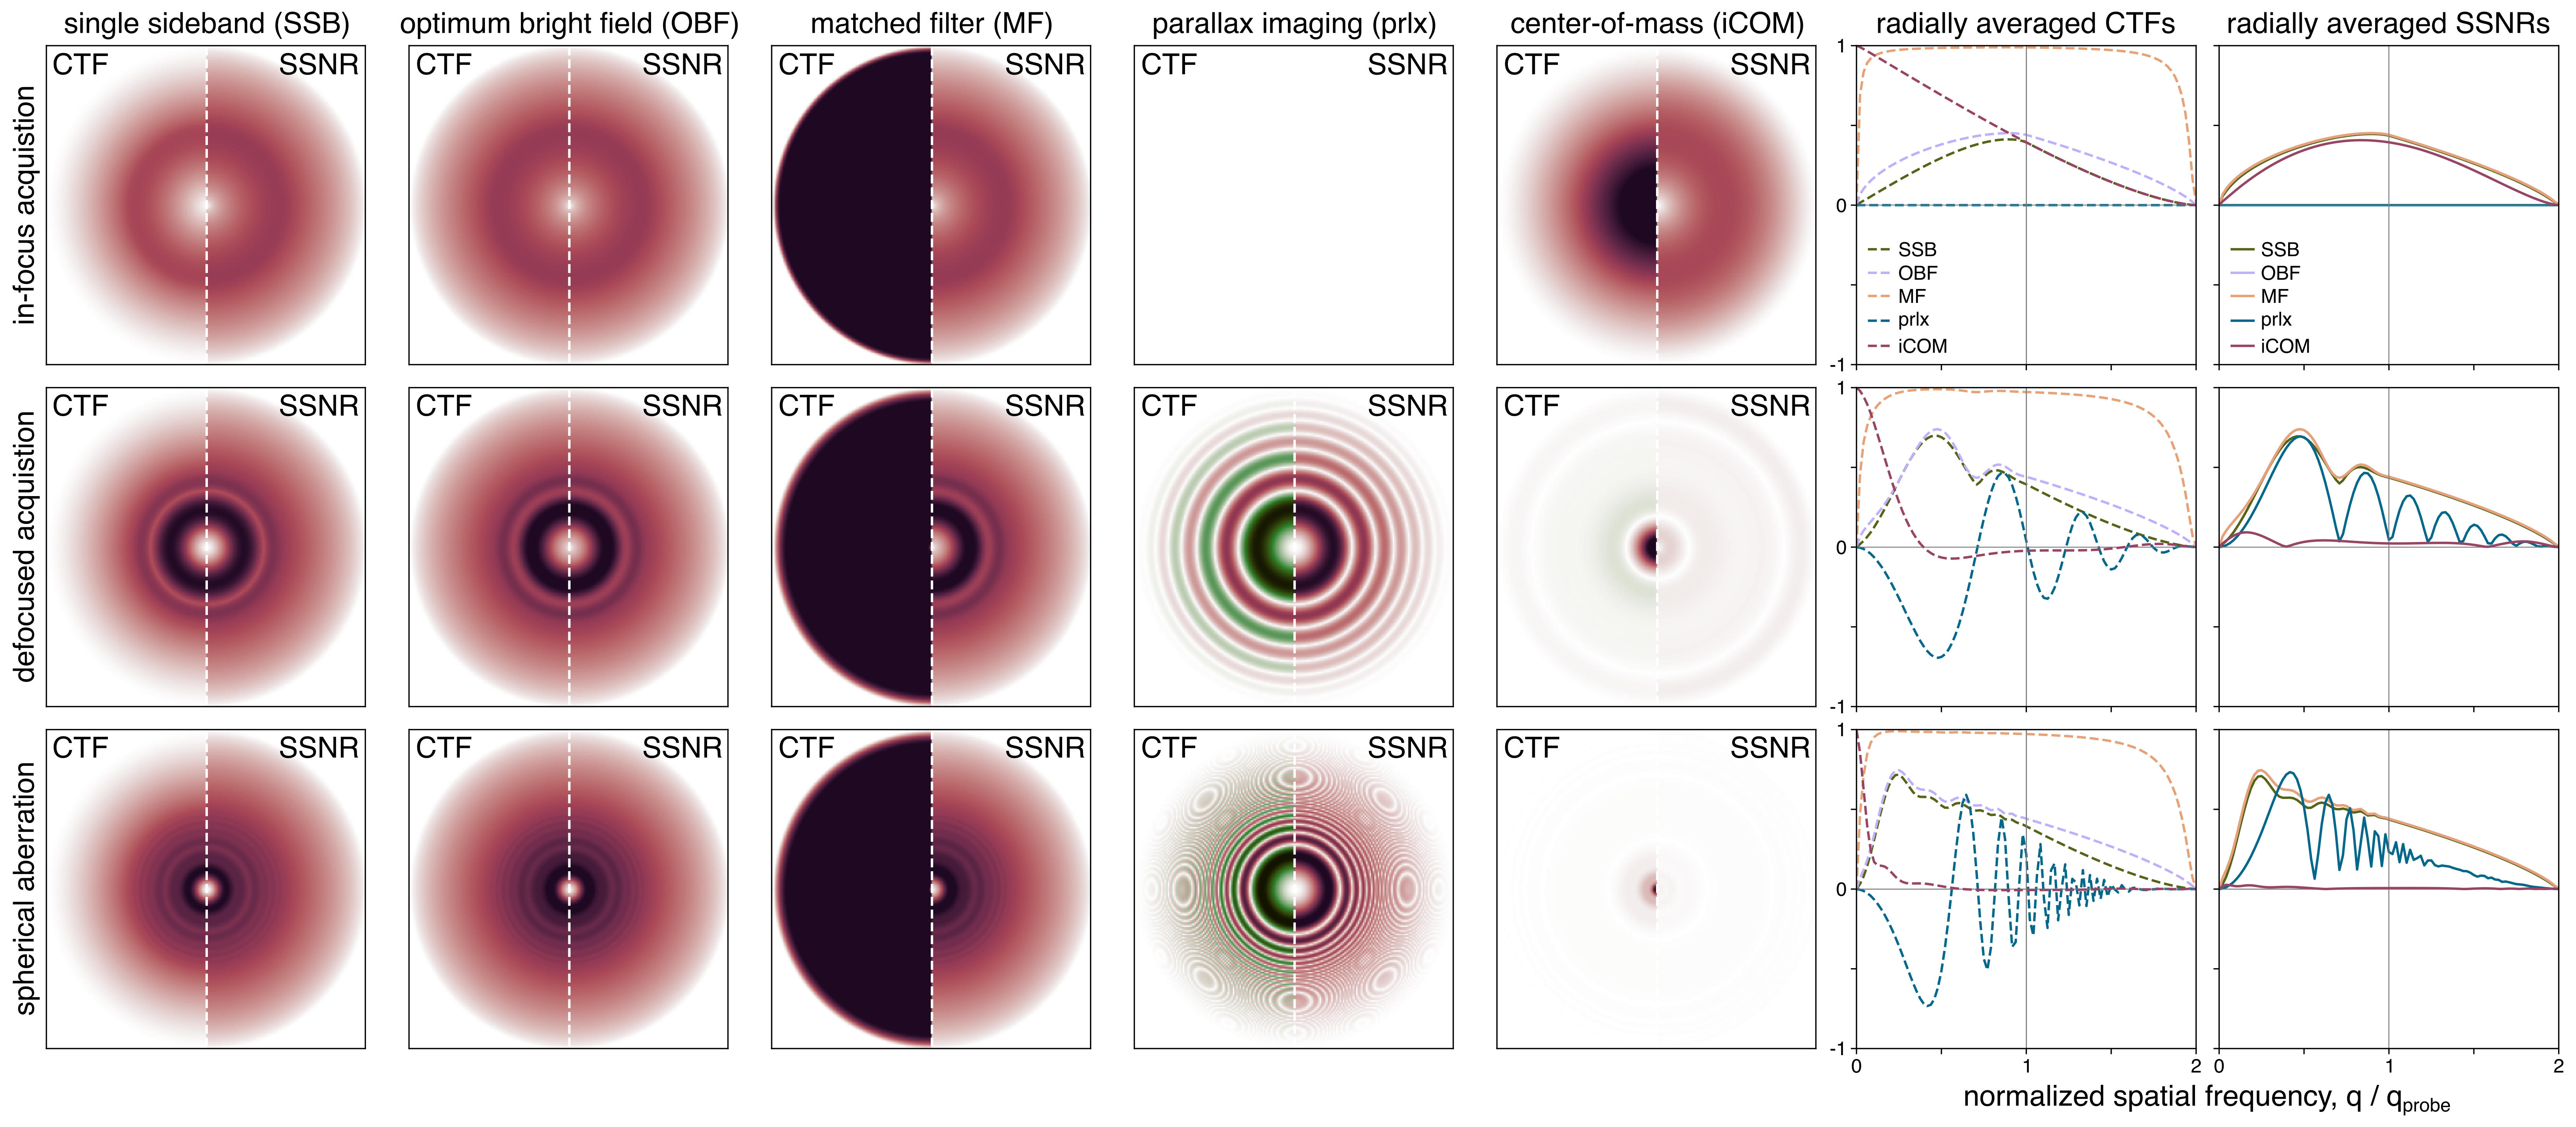
\includegraphics[width=\textwidth]{raster/direct-ctf-figure.png}
  \caption{Contrast transfer functions (CTFs) and spectral signal-to-noise ratios (SSNRs) for all direct techniques investigated across different acquisition parameters, highlighting the SSNR equivalence for SSB, OBF, and MF/WDD.}
  \label{fig:ctf}
\end{figure*}

\DIFdelbegin \subsection{\DIFdel{Phase-Compensated Coherent Sum}}
%DIFAUXCMD
\addtocounter{subsection}{-1}%DIFAUXCMD
\DIFdelend \DIFaddbegin \subsection*{\DIFadd{Phase-compensated coherent sum}}
\DIFaddend \label{sec:ssb}

The first technique we investigate goes by two seemingly unrelated names: \emph{aberration-corrected bright-field (acBF) STEM}~\cite{Ma_2025} and \emph{phase-compensated single-sideband (SSB) ptychography}~\cite{Yang_2016}.
The former highlights its close connection to \emph{tilt-corrected bright-field (tcBF) STEM}, which we investigate further in the Quadratic Approximation section.
The latter name reflects the structure of the WPOA forward model in \cref{eq:wpoa-forward}, which contains two redundant contributions at $\boldsymbol{q}$ and $-\boldsymbol{q}$.

In the absence of aberrations, these two ``sidebands\DIFdelbegin \DIFdel{'' are related by complex conjugation according to Friedel'}\DIFdelend \DIFaddbegin \DIFadd{" provide complex-conjugate estimates of the same object Fourier component, consistent with Friedel’}\DIFaddend s law.\footnote{Friedel's law illustrates how a single mathematical principle -- the Hermitian conjugation symmetry of the Fourier transform of a real-valued function -- connects the physics of imaging with crystallographic structure determination~\cite{Friedel_1913,karle1985}.}
Accordingly, the specimen phase $\tilde{\phi}(\boldsymbol{q})$ can be reconstructed using only one of them.
In practice, once aberrations are present, the two \DIFdelbegin \DIFdel{sidebands are no longer perfect conjugates: residual aberrations imprint an additional geometric phase on the aperture-overlap function $\Gamma(\boldsymbol{q},\boldsymbol{k})$.
}\DIFdelend \DIFaddbegin \DIFadd{overlap regions acquire different geometric phase factors arising from the probe aberration function $\chi(\boldsymbol{k})$.
As a result, they no longer correspond to simple complex-conjugate estimates of the same object Fourier component.
}\DIFaddend 

The key insight behind SSB is that, under the WPOA, detector pixels sampling the same sideband carry the same specimen phase $\tilde{\phi}(\boldsymbol{q})$.
Differences between pixels arise only from known, instrument-dependent phases, namely aberration-induced geometric phases and aperture-overlap geometry.
If these extra phases are removed, sideband contributions from all detector pixels can be added coherently.

Phase-compensated SSB accomplishes this by dividing $\Gamma(\boldsymbol{q},\boldsymbol{k})$ by its magnitude and retaining only its phase factor, effectively rotating each detector-plane frequency into a common phase reference.
The estimated phase is then obtained by coherently summing all phase-aligned detector samples~\cite{Yang_2016}:
\begin{equation}
  \tilde{\phi}_{\text{SSB}}(\boldsymbol{q}) = \sum_{\boldsymbol{k}} \frac{\Gamma^{*}(\boldsymbol{q},\boldsymbol{k})\,G(\boldsymbol{q},\boldsymbol{k})}{\lvert \Gamma(\boldsymbol{q},\boldsymbol{k}) \rvert}.
  \label{eq:ssb-recon}
\end{equation}

\Cref{eq:ssb-recon} works remarkably well and remains one of the most widely used direct phase-retrieval techniques.
Inserting the forward model $G(\boldsymbol{q},\boldsymbol{k})=\Gamma(\boldsymbol{q},\boldsymbol{k})\tilde{\phi}(\boldsymbol{q})$ into \cref{eq:ssb-recon} gives the SSB CTF~\cite{Yang_2016}
\begin{equation}
  \mathrm{CTF}_{\text{SSB}}(\boldsymbol{q}) = \frac{i}{2} \sum_{\boldsymbol{k}} \lvert \Gamma(\boldsymbol{q},\boldsymbol{k}) \rvert.
  \label{eq:ctf-ssb}
\end{equation}
For spatial frequencies beyond the aperture semiangle, $\lvert \boldsymbol{q} \rvert > q_0$, the overlap $\Gamma(\boldsymbol{q},\boldsymbol{k})$ reduces to the double-overlap region, and the CTF collapses to the ideal autocorrelation envelope in \cref{eq:infocus-ctf}.

To understand the SSB variance, note that each detector frequency contributes a noisy measurement,
\begin{equation}
  G(\boldsymbol{q},\boldsymbol{k}) = \Gamma(\boldsymbol{q},\boldsymbol{k})\tilde{\phi}(\boldsymbol{q}) + n(\boldsymbol{q},\boldsymbol{k}),
  \label{eq:noise-model}
\end{equation}
with unit-variance noise $n(\boldsymbol{q},\boldsymbol{k})$~\cite{Bennemann_2025}.
The phase-alignment step preserves unit variance, so noise contributions add incoherently while the signal adds coherently.
Thus, the total variance at each spatial frequency $\boldsymbol{q}$ is simply the number of detector pixels for which $\Gamma(\boldsymbol{q},\boldsymbol{k})$ is nonzero:
\begin{align}
  \operatorname{Var}\!\left[\tilde{\phi}_{\text{SSB}}(\boldsymbol{q})\right] &= \sum_{\boldsymbol{k}} \mathbf{1}_{\{\lvert \Gamma(\boldsymbol{q},\boldsymbol{k}) \rvert > 0\}} \nonumber\\
  &= 2 D(\boldsymbol{q})+T(\boldsymbol{q}), 
  \label{eq:var-ssb}
\end{align}
where $D(\boldsymbol{q})$ and $T(\boldsymbol{q})$ are the double- and triple-overlap regions (\cref{fig:gamma}).
The resulting SSNR is~\cite{Bennemann_2025,Varnavides_2025_ssnr}
\begin{equation}
  \mathrm{SSNR}_{\text{SSB}}(\boldsymbol{q}) = \frac{\sum_{\boldsymbol{k}}\lvert \Gamma(\boldsymbol{q},\boldsymbol{k}) \rvert}{2\sqrt{2D(\boldsymbol{q})+T(\boldsymbol{q})}} .
  \label{eq:ssb-ssnr}
\end{equation}

\DIFdelbegin \subsection{\DIFdel{Noise-Flattening Normalization}}
%DIFAUXCMD
\addtocounter{subsection}{-1}%DIFAUXCMD
\DIFdelend \DIFaddbegin \begin{figure*}[t]
  \centering
  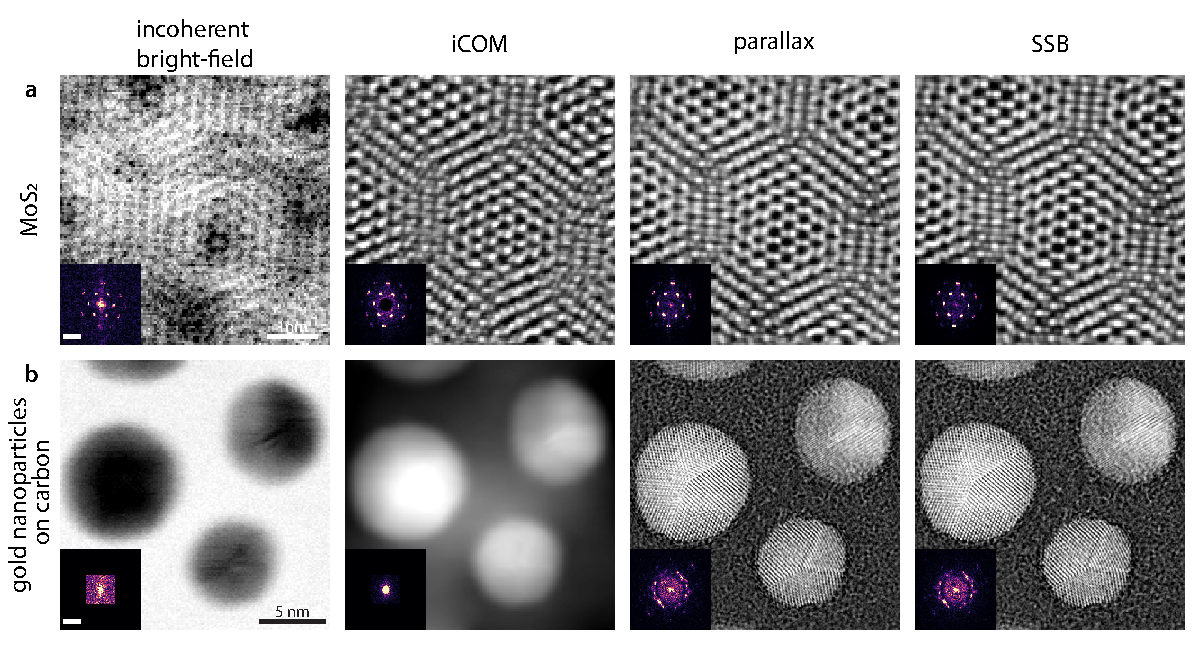
\includegraphics[width=\textwidth]{vector/direct_gold_mos2.pdf}
  \caption{\DIFaddFL{Direct-method reconstructions for (a)~near-focus MoS$_2$ acquisition~\mbox{%DIFAUXCMD
\cite{zhang2025atom} }\hskip0pt%DIFAUXCMD
and (b)~defocused gold nanoparticle datasets.}}
  \label{fig:exp-compare}
\end{figure*}

\subsection*{\DIFadd{Noise-flattening normalization}}
\DIFaddend \label{sec:obf}

Phase-compensated SSB improves robustness against residual aberrations by removing the geometric phase of the aperture-overlap function before summing detector-plane frequencies.
However, SSB still treats all contributing detector pixels equally, even though the strength of the aperture overlap varies strongly across the bright-field disk, resulting in a statistically sub-optimal reconstruction.

The \emph{optimum bright-field (OBF) STEM} method addresses this by applying a noise-matched normalization to the SSB estimator~\cite{Ooe_2021,Ooe_2024}.
Starting from the phase-aligned numerator, OBF introduces a scalar normalization factor proportional to the root-mean-squared aperture-overlap strength:
\begin{equation}
  \tilde{\phi}_{\text{OBF}}(\boldsymbol{q}) = \frac{\sum_{\boldsymbol{k}} \Gamma^{*}(\boldsymbol{q},\boldsymbol{k})\,G(\boldsymbol{q},\boldsymbol{k})}{\sqrt{\sum_{\boldsymbol{k}}\lvert \Gamma(\boldsymbol{q},\boldsymbol{k}) \rvert^2}} .
  \label{eq:obf-recon}
\end{equation}

The denominator rescales the coherent SSB sum by the effective SSNR of the bright-field detector region.
For each spatial frequency, this normalization prevents a small subset of bright-field pixels with weak overlap from amplifying noise.
Thus, OBF can be viewed as a noise-flattened SSB formulation, retaining geometric phase compensation but adjusting its gain to reflect information reliability.

Substituting the WPOA forward model into \cref{eq:obf-recon} gives
\begin{equation}
  \mathrm{CTF}_{\text{OBF}}(\boldsymbol{q}) = \frac{i}{2} \sqrt{\sum_{\boldsymbol{k}}\lvert \Gamma(\boldsymbol{q},\boldsymbol{k}) \rvert^2}.
  \label{eq:obf-ctf}
\end{equation}

Using the additive unit-variance noise model in \cref{eq:noise-model}, the numerator becomes
\begin{align}
  \sum_{\boldsymbol{k}}\Gamma^{*}(\boldsymbol{q},\boldsymbol{k})G(\boldsymbol{q},\boldsymbol{k}) &=
  \sum_{\boldsymbol{k}}\lvert \Gamma(\boldsymbol{q},\boldsymbol{k}) \rvert^2 \tilde{\phi}(\boldsymbol{q}) \nonumber\\
  &\quad + \sum_{\boldsymbol{k}}\Gamma^{*}(\boldsymbol{q},\boldsymbol{k})n(\boldsymbol{q},\boldsymbol{k}),
  \label{eq:obf-numerator}
\end{align}
with variance
\begin{equation}
  \operatorname{Var}\!\left[ \sum_{\boldsymbol{k}}\Gamma^{*}(\boldsymbol{q},\boldsymbol{k})n(\boldsymbol{q},\boldsymbol{k}) \right] = \sum_{\boldsymbol{k}}\lvert \Gamma(\boldsymbol{q},\boldsymbol{k}) \rvert^2 .
  \label{eq:obf-var}
\end{equation}
This is precisely the OBF denominator squared, thus normalizing the OBF variance to unity, $\operatorname{Var}[\tilde{\phi}_{\text{OBF}}(\boldsymbol{q})]=1$.
The resulting OBF SSNR is thus given simply by the magnitude of its CTF
\begin{equation}
  \mathrm{SSNR}_{\text{OBF}}(\boldsymbol{q}) = \frac{1}{2} \sqrt{\sum_{\boldsymbol{k}}\lvert \Gamma(\boldsymbol{q},\boldsymbol{k}) \rvert^2}.
  \label{eq:obf-ssnr}
\end{equation}

\DIFdelbegin %DIFDELCMD < \begin{figure*}[t]
%DIFDELCMD <   \centering
%DIFDELCMD <   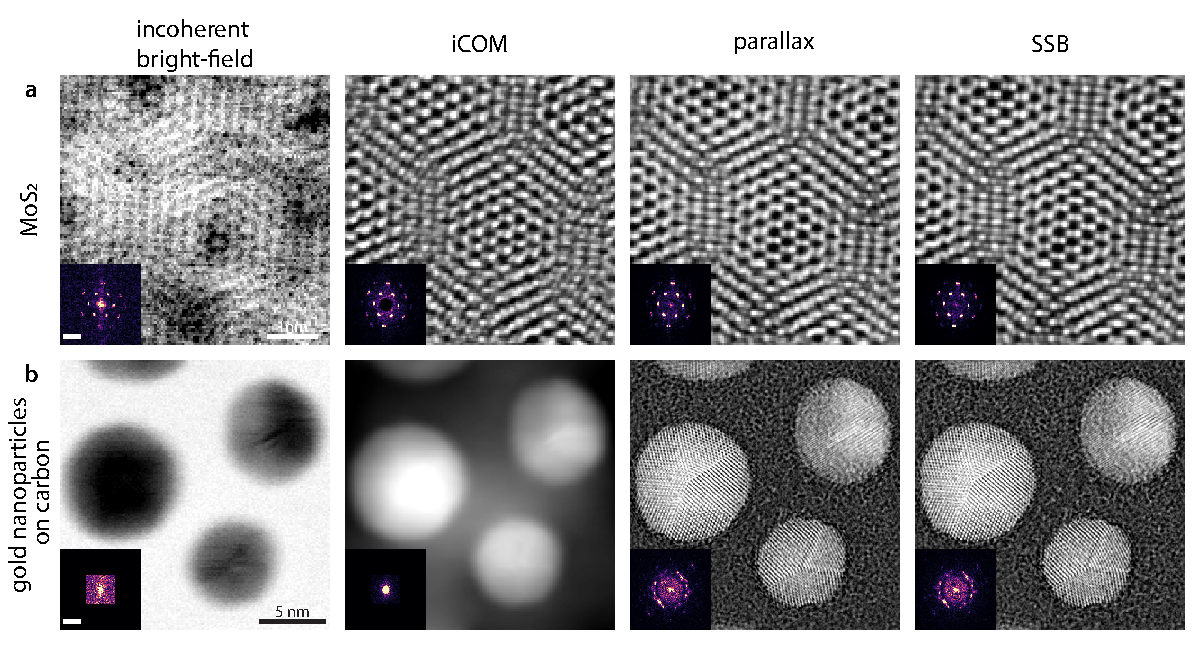
\includegraphics[width=\textwidth]{vector/direct_gold_mos2.pdf}
%DIFDELCMD <   %%%
%DIFDELCMD < \caption{%
{%DIFAUXCMD
\DIFdelFL{Direct-method reconstructions for (a)~near-focus MoS$_2$ acquisition~\mbox{%DIFAUXCMD
\cite{zhang2025atom} }\hskip0pt%DIFAUXCMD
and (b)~defocused gold nanoparticle datasets.}}
  %DIFAUXCMD
%DIFDELCMD < \label{fig:exp-compare}
%DIFDELCMD < \end{figure*}
%DIFDELCMD < 

%DIFDELCMD < %%%
\subsection{\DIFdel{Least-Squares Matched Filter}}
%DIFAUXCMD
\addtocounter{subsection}{-1}%DIFAUXCMD
\DIFdelend \DIFaddbegin \subsection*{\DIFadd{Least-squares matched filter}}
\DIFaddend \label{sec:wdd}

The OBF estimator above improves SSB by normalizing the coherent sum, but it is not formally a least-squares estimator.
The proper matched-filter (MF) solution for recovering $\tilde(\phi)(\boldsymbol{q})$ from the WPOA forward model is obtained by minimizing $\sum_{\boldsymbol{k}}\lvert G(\boldsymbol{q},\boldsymbol{k})-\Gamma(\boldsymbol{q},\boldsymbol{k})\tilde{\phi}(\boldsymbol{q}) \rvert^2$, yielding the estimator
\begin{equation}
  \tilde{\phi}_{\text{MF}}(\boldsymbol{q}) = 
  \frac{\sum_{\boldsymbol{k}} \Gamma^{*}(\boldsymbol{q},\boldsymbol{k})\,G(\boldsymbol{q},\boldsymbol{k})}{\sum_{\boldsymbol{k}}\lvert \Gamma(\boldsymbol{q},\boldsymbol{k}) \rvert^2 + \epsilon(\boldsymbol{q})}.
  \label{eq:mf-recon}
\end{equation}

While~\cref{eq:mf-recon} is simple, direct evaluation in detector-space is numerically unstable:
the numerator contains highly oscillatory phases from $\Gamma(\boldsymbol{q},\boldsymbol{k})$, and the denominator depends on the squared magnitude of a rapidly varying overlap kernel.
Applying Parseval's theorem, $\sum_k \lvert \tilde{f}(k)\rvert^2 = \int d r \lvert f(r)\rvert^2$, and inverse Fourier transforming over $\boldsymbol{k}$ gives the MF estimator in the mixed-domain representation
\begin{align}
\tilde{\phi}_{\text{MF-mix}}(\boldsymbol{q})
&=
\frac{\int W^{*}(\boldsymbol{q},\boldsymbol{\rho})H(\boldsymbol{q},\boldsymbol{\rho})\,\mathrm{d}\boldsymbol{\rho}}{\int \lvert W(\boldsymbol{q},\boldsymbol{\rho}) \rvert^2\,\mathrm{d}\boldsymbol{\rho}+\epsilon(\boldsymbol{q})},
\label{eq:mf-mixed-recon}
\\
W(\boldsymbol{q},\boldsymbol{\rho})
&=
\mathcal{F}^{-1}\{\Gamma(\boldsymbol{q},\boldsymbol{k})\},
\label{eq:wigner-w}
\\
H(\boldsymbol{q},\boldsymbol{\rho})
&=
\mathcal{F}^{-1}\{G(\boldsymbol{q},\boldsymbol{k})\},
\label{eq:wigner-h}
\end{align}
where $\boldsymbol{\rho}$ is the detector separation.
This utilizes the fact that the kernel $W(\boldsymbol{q},\boldsymbol{\rho})$ is highly-localized in $\rho$, suggesting that we can further improve numerical stability by switching to a pixelwise normalization
\begin{equation}
\tilde{\phi}_{\text{WDD}}(\boldsymbol{q})=
\int \frac{ W^{*}(\boldsymbol{q},\boldsymbol{\rho})H(\boldsymbol{q},\boldsymbol{\rho})}{\lvert W(\boldsymbol{q},\boldsymbol{\rho}) \rvert^2+\epsilon(\boldsymbol{q},\boldsymbol{\rho})}\,\mathrm{d}\boldsymbol{\rho},
\label{eq:wdd-recon}
\end{equation}
which is commonly referred to as the \emph{Wigner distribution deconvolution (WDD)} method~\cite{Rodenburg_1992,Li_2014,Yang_2017}.
Similar to SSB, usually only one of the sidebands is used to form the kernel $W(\boldsymbol{q},\boldsymbol{\rho}) = \mathcal{F}^{-1}\{\tilde{\psi}(\boldsymbol{k-q})\tilde{\psi}^{*}(\boldsymbol{k})\}$.

The MF (and equivalently WDD) estimator can be characterized by a contrast transfer function by inserting the forward model into~\cref{eq:mf-recon}
\begin{equation}
\mathrm{CTF}_{\text{MF}}(\boldsymbol{q})
=
\frac{\sum_{\boldsymbol{k}}\lvert \Gamma(\boldsymbol{q},\boldsymbol{k}) \rvert^2}{\sum_{\boldsymbol{k}}\lvert \Gamma(\boldsymbol{q},\boldsymbol{k}) \rvert^2+\epsilon(\boldsymbol{q})},
\label{eq:mf-ctf}
\end{equation}
Note that for sufficiently small regularization $\epsilon(\boldsymbol{q})$, the matched-filter CTF approaches unity, implying perfect phase transfer.
This is misleading, since the MF noise variance is similarly increased
\begin{equation}
\operatorname{Var}\!\left[\tilde{\phi}_{\text{MF}}(\boldsymbol{q})\right]
=
\frac{\operatorname{Var}\!\left[\tilde{\phi}_{\text{OBF}}(\boldsymbol{q})\right]}{\sum_{\boldsymbol{k}}\lvert \Gamma(\boldsymbol{q},\boldsymbol{k}) \rvert^2}
=
\frac{1}{\sum_{\boldsymbol{k}}\lvert \Gamma(\boldsymbol{q},\boldsymbol{k}) \rvert^2},
\label{eq:mf-var}
\end{equation}
to obtain an SSNR which is identical to that of OBF
\begin{equation}
\mathrm{SSNR}_{\text{MF}}(\boldsymbol{q})
=
\frac{1}{2}
\sqrt{\sum_{\boldsymbol{k}}\lvert \Gamma(\boldsymbol{q},\boldsymbol{k}) \rvert^2}.
\label{eq:mf-ssnr}
\end{equation}

This highlights an important subtlety: the statistically-reliable information content is effectively the same for all three linear estimators we have explored so far, namely SSB, OBF, and MF/WDD.

\DIFdelbegin \subsection{\DIFdel{Quadratic Approximation}} %DIFAUXCMD
\addtocounter{subsection}{-1}%DIFAUXCMD
\DIFdelend \DIFaddbegin \subsection*{\DIFadd{Quadratic approximation}} \DIFaddend \label{sec:parallax}

The methods we have introduced so far all relied on the full aperture-overlap kernel $\Gamma(\boldsymbol{q},\boldsymbol{k})$, which is expensive to compute numerically.
A natural question is whether a computationally efficient approximation exists that retains most of the information.

The \emph{tilt-corrected bright-field (tcBF) STEM}~\cite{Nguyen_2016,Spoth_2017,Yu_2025} or \emph{parallax imaging}~\cite{Varnavides_2023,Varnavides_2024,Varnavides_2025} method originated independently, based on the reciprocity principle.
Specifically, a virtual bright-field image formed form a given nonzero detector frequency during a defocused acquisition will appear laterally shifted in real space.
Computationally reversing this parallax effect, with subpixel accuracy using a detector-frequency-dependent phase ramp, restores all virtual BF images into a common focal plane, where they can be coherently summed~\cite{Yu_2025,Varnavides_2025}.

Formally, this parallax correction is equivalent to applying a phase factor $\exp[i \nabla_{\boldsymbol{k}} \chi(\boldsymbol{k}) \cdot \boldsymbol{q}]$ to the virtual bright-field images, where $\nabla_{\boldsymbol{k}} \chi(\boldsymbol{k})$ is the gradient of the aberration surface at bright field frequency $\boldsymbol{k}$.
To see the connection with SSB explicitly, we Taylor-expand $\Gamma(\boldsymbol{q},\boldsymbol{k})$ to first order in $\boldsymbol{q}$
\begin{align}
\Gamma(\boldsymbol{q},\boldsymbol{k})
&\approx
B(\boldsymbol{q},\boldsymbol{k})
\exp\!\left[i\nabla_{\boldsymbol{k}}\chi(\boldsymbol{k})\cdot\boldsymbol{q}\right],
\\
B(\boldsymbol{q},\boldsymbol{k})
&=
A(\boldsymbol{k})
\Big[
A(\boldsymbol{q}-\boldsymbol{k})e^{-i\chi(\boldsymbol{q})}
-
A(\boldsymbol{q}+\boldsymbol{k})e^{i\chi(\boldsymbol{q})}
\Big].
\label{eq:prlx-gamma-approx}
\end{align}

where $B(\boldsymbol{q},\boldsymbol{k})$ contains the aperture-overlap terms, while the remaining factor produces the parallax shift.
Thus, parallax imaging can be seen as a quadratic approximation to SSB, where only the first-order-aberrations-induced phase ramp is retained.

Combined with a global phase-flipping operation, parallax imaging provides a remarkably robust and computationally efficient approximation to SSB~\cite{Varnavides_2025}
\begin{equation}
\tilde{\phi}_{\text{prlx}}(\boldsymbol{q})
=
\sum_{\boldsymbol{k}}
G(\boldsymbol{q},\boldsymbol{k})
\,\operatorname{sgn}[\sin\chi(\boldsymbol{q})]\,
e^{-i\nabla_{\boldsymbol{k}}\chi(\boldsymbol{k})\cdot\boldsymbol{q}} .
\label{eq:par-recon}
\end{equation}

The corresponding CTF is obtained by summing the omitted kernel $B(\boldsymbol{q},\boldsymbol{k})$ over the bright-field disk
\begin{align}
\mathrm{CTF}_{\text{prlx}}(\boldsymbol{q})
&=
\frac{i}{2}\sum_{\boldsymbol{k}}B(\boldsymbol{q},\boldsymbol{k})
\nonumber\\
&=
-i\,\sin[\chi(\boldsymbol{q})]\,[A\star A](\boldsymbol{q}),
\label{eq:prlx-ctf}
\end{align}
which reduces to the axial-illumination CTF, modulated by the aperture autocorrelation function~\cite{Yu_2022,Varnavides_2024,Varnavides_2025}.

Since the parallax estimator simply shifts each virtual bright-field image before coherently summing, the noise contributions retain unit variance.
Consequently, $\operatorname{Var}\!\left[\tilde{\phi}_{\text{prlx}}(\boldsymbol{q})\right]=1$ and the parallax SSNR is
\begin{equation}
\mathrm{SSNR}_{\text{prlx}}(\boldsymbol{q})
=
\lvert \sin[\chi(\boldsymbol{q})] \rvert\,[A\star A](\boldsymbol{q}).
\label{eq:prlx-ssnr}
\end{equation}

\begin{figure}
  \centering
  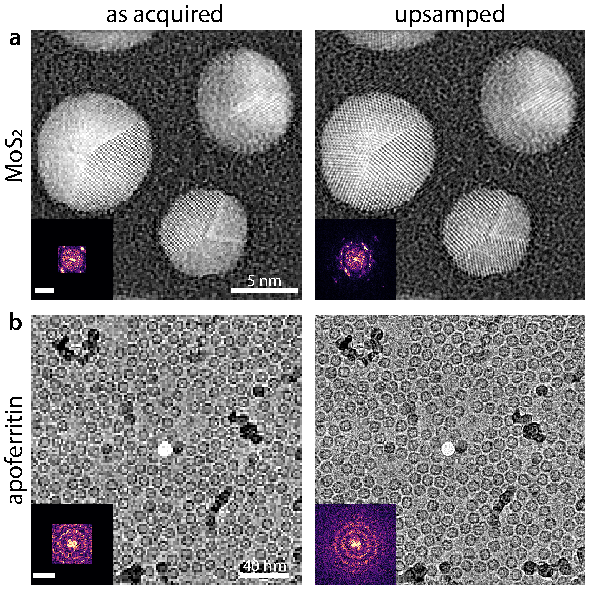
\includegraphics[width=\linewidth]{vector/upsample.pdf}
  \caption{Upsampled
  \textit{(a)} gold nanoparticles and \textit{(b)} apoferritin~\cite{Berk_2024} parallax imaging reconstructions.}
  \label{fig:uspsample}
\end{figure}

\DIFdelbegin \subsection{\DIFdel{First-Moment Projection}}
%DIFAUXCMD
\addtocounter{subsection}{-1}%DIFAUXCMD
\DIFdelend \DIFaddbegin \subsection*{\DIFadd{First-moment projection}}
\DIFaddend \label{sec:icom}

An alternative and computationally efficient route to STEM phase retrieval is to take the first moment of the aperture–overlap function, known either as \emph{integrated center-of-mass (iCOM) imaging} or \emph{integrated differential phase contrast (iDPC or DPC)}~\cite{Dekkers_1974,Lazic_2016}.
Compared to other direct approaches, these are the most computationally-efficient and straightforward, although they do not provide the same aberration deconvolution advantages discussed above for the other direct approaches.

Starting from the WPOA CTF expression in~\cref{eq:ctf} and using a vectorial detector response $D(\boldsymbol{k}) = \boldsymbol{k}$, we obtain the vector COM transfer function as

\begin{align}
\mathrm{CTF}_{\text{COM}}(\boldsymbol{q})
&=
\frac{i}{2}\int \Gamma(\boldsymbol{q},\boldsymbol{k})\,\boldsymbol{k}\,\mathrm{d}\boldsymbol{k}
\nonumber\\
&=
\frac{i\boldsymbol{q}}{2}[\tilde{\psi}\star\tilde{\psi}](\boldsymbol{q}).
\label{eq:com-ctf}
\end{align}
i.e. the first moment of $\Gamma(\boldsymbol{q},\boldsymbol{k})$ which is proportional to the probe autocorrelation weighted by $\boldsymbol{q}$.

Fourier differentiation satisfies $\mathcal{F}_{\boldsymbol{r} \rightarrow \boldsymbol{q}}\{\nabla_{\boldsymbol{r}} \phi(\boldsymbol{r})\} = i \, \boldsymbol{q} \; \tilde{\phi}(\boldsymbol{q})$, and thus we recognize the measured COM signal as a filtered estimate of the phase gradient, with the filter given by the probe autocorrelation.
To obtain the specimen phase, we Fourier-integrate the vector COM measurement to obtain:
\begin{equation}
\tilde{\phi}_{\text{iCOM}}(\boldsymbol{q})
=
\sum_{\boldsymbol{k}} \frac{\boldsymbol{q}\cdot[G(\boldsymbol{q},\boldsymbol{k})\,\boldsymbol{k}]}{i\lvert \boldsymbol{q} \rvert^2},
\label{eq:icom-recon}
\end{equation}
Applying the same integration to the vectorial CTF yields the scalar iCOM transfer function
\begin{equation}
\mathrm{CTF}_{\text{iCOM}}(\boldsymbol{q})
=
i[\tilde{\psi}\star\tilde{\psi}](\boldsymbol{q}),
\label{eq:icom-ctf}
\end{equation}
highlighting that iCOM reconstructs the specimen phase convolved with the probe autocorrelation~\cite{Bekkevold_2025}.

The COM signal division by the spatial frequency, suggests the noise in the reconstruction scales with $\lvert\boldsymbol{q}\rvert$, to give the iCOM SSNR as~\cite{Varnavides_2025_ssnr}
\begin{equation}
\mathrm{SSNR}_{\text{iCOM}}(\boldsymbol{q})
=
\frac{\lvert [\tilde{\psi}\star\tilde{\psi}](\boldsymbol{q}) \rvert}{\lvert \boldsymbol{q} \rvert}.
\label{eq:icom-ssnr}
\end{equation}

\Cref{eq:icom-ssnr} highlights that while the iCOM CTF suggests low spatial frequencies transfer with unit contrast, the corresponding SSNR shows these components become increasingly noisy in practice~\cite{Varnavides_2023,Yu_2025,Varnavides_2025_ssnr}.

\DIFdelbegin \subsection{\DIFdel{Comparison of Direct Techniques}}
%DIFAUXCMD
\addtocounter{subsection}{-1}%DIFAUXCMD
\DIFdelend \DIFaddbegin \subsection*{\DIFadd{Comparison of direct techniques}}
\DIFaddend 

The phase estimators introduced above -- SSB, OBF, MF/WDD, parallax, and iCOM -- all originate from the same WPOA forward model in \cref{eq:wpoa-forward} and additive noise model in \cref{eq:noise-model}.
They primarily differ in (i) how they weight the bright-field intensities, (ii) how they normalize the coherent sum, and (iii) how much of the aperture-overlap kernel they retain.

SSB performs an unnormalized coherent projection using the full aperture-overlap kernel.
OBF applies a noise-flattening scalar normalization.
MF/WDD implements the least-squares matched filter, either in detector space (MF) or in a mixed domain (WDD).
Parallax imaging uses a first-order approximation to the aperture-overlap kernel, keeping only the detector-frequency-dependent phase ramp
\(
\exp\!\left[i \nabla_{\boldsymbol{k}}\chi(\boldsymbol{k}) \cdot \boldsymbol{q}\right],
\)
making it computationally cheap.
Parallax subpixel shift estimation accuracy enables scan step-size upsampling (\cref{fig:uspsample}), although this can be extended to other direct methods as well~\cite{Varnavides_2025}.
\DIFaddbegin \DIFadd{The impact of upsampling is demonstrated in~\mbox{%DIFAUXCMD
\cref{fig:uspsample} }\hskip0pt%DIFAUXCMD
by comparing the left and right columns, where computational upsampling leads to a clear improvement in spatial resolution and feature definition. 
}\DIFaddend Finally, iCOM bypasses the overlap kernel entirely, and instead takes the first moment of the bright-field intensities and reconstructs the phase by Fourier integration of the resulting COM signal.

With the exception of iCOM, these techniques rely on an accurate estimation of the aberrations, which can be calculated through optimization routines based on self-consistency error~\cite{Varnavides_2025}, or by least-squares fitting of linear systems of equations~\cite{Varnavides_2023,Yu_2025}.

\Cref{unified-pseudocode} shows a unified pseudocode for the direct estimators we have seen so far, using a loop over bright-field pixels $\boldsymbol{k}_{\mathrm{BF}}$.
This leverages the fact that the aperture-overlap function is identically zero outside the probe aperture, making it computationally efficient, and enabling natural upsampling via Fourier tiling~\cite{Varnavides_2025}.
It should be noted that, due to the mixed-domain requirement, WDD cannot be computed by solely looping over $\boldsymbol{k}_{\mathrm{BF}}$.

As highlighted in\DIFaddbegin \DIFadd{~}\DIFaddend \cref{fig:ctf,fig:exp-compare}, the ideal approach depends on the nature of the data and acquisition parameters.
For in-focus experiments, iCOM is often the preferred approach, with the low computational overhead of this technique making it most compatible with \textit{in situ} approaches~\cite{bekkevold2024ultra}.
\DIFdelbegin \DIFdel{Conversely, parallax reconstructions are often performed for defocused acquisitions using large step sizes, e.g., for beam-sensitive biological samples~\mbox{%DIFAUXCMD
\cite{Berk_2024,Yu_2025}}\hskip0pt%DIFAUXCMD
}\DIFdelend \DIFaddbegin \DIFadd{This behavior is evident in~\mbox{%DIFAUXCMD
\cref{fig:ctf,fig:exp-compare}}\hskip0pt%DIFAUXCMD
a, where all phase-retrieval methods yield comparable reconstructions due to the high sampling and near in-focus acquisition conditions.
The advantage of parallax and direct ptychography becomes apparent in the defocused dataset (\mbox{%DIFAUXCMD
\cref{fig:ctf,fig:exp-compare}}\hskip0pt%DIFAUXCMD
b), where only these approaches recover atomic-scale information.
Notably, the reconstruction quality of parallax closely matches that of single-sideband (SSB), consistent with its interpretation as a quadratic approximation to the full phase-compensated inversion}\DIFaddend .

The SSB, OBF, and MF/WDD techniques \DIFdelbegin \DIFdel{perform a full deconvolution of the aperture overlap and are also suited for acquisitions with }\DIFdelend \DIFaddbegin \DIFadd{compensate for the aperture-overlap transfer function using knowledge of the probe wavefunction, allowing recovery of the object phase even in the presence of }\DIFaddend residual higher-order \DIFdelbegin \DIFdel{aberration}\DIFdelend \DIFaddbegin \DIFadd{aberrations}\DIFaddend ~\cite{Varnavides_2025,Susi_2025}.
\DIFaddbegin \DIFadd{MF/WDD performs this compensation through an explicit Wiener deconvolution, while SSB and OBF incorporate the probe phase directly into their reconstruction kernels.
}\DIFaddend However, ptychographic acquisitions on aberration-corrected instruments are often dominated by \DIFdelbegin \DIFdel{first-order }\DIFdelend \DIFaddbegin \DIFadd{low-order }\DIFaddend aberrations such as defocus and astigmatism\DIFdelbegin \DIFdel{, suggesting the quadratic approximation provided by parallax yields a nearly identical reconstruction as }\DIFdelend \DIFaddbegin \DIFadd{. 
In this regime, the quadratic phase approximation underlying parallax provides an effective description of the probe phase, yielding reconstructions that are nearly identical to those obtained with }\DIFaddend SSB, OBF, or MF/WDD~\cite{Varnavides_2025_ssnr}.

For low-dose experiments, the direct phase-retrieval techniques perform remarkably well as compared to their more computationally expensive counterparts~\cite{Varnavides_2025_ssnr}, suggesting that more advanced reconstruction approaches may not be needed offline.
However, for thick samples and experiments with higher electron fluence, iterative approaches outperform their direct phase retrieval counterparts as described in the Iterative Ptychography section.

\begin{figure}
\renewcommand{\figurename}{Algorithm}
\hrule \vspace{5pt}
\caption{Unified direct STEM phase retrieval}
\vspace{5pt} \hrule \vspace{5pt}
\label{unified-pseudocode}
\begin{algorithmic}

\Statex \textbf{Inputs:}
\Statex \quad 4D-STEM dataset $I(\boldsymbol{r},\boldsymbol{k})$
\Statex \quad estimator type $\in\{\text{SSB},\text{OBF},\text{MF},\text{prlx},\text{iCOM}\}$
\Statex \quad integer upsampling factor $f$
\Statex \quad aberration coefficients $C_{n,m}$ (for $\chi$ and $\nabla_{\boldsymbol{k}}\chi$)
\Statex \quad convergence semiangle $k_0$
\Statex \quad scan/detector rotation angle $\theta$

\Statex \textbf{Output:} estimated phase upsampled by factor $f$

\Statex
\Statex \textbf{Initialization:}
\Statex Allocate $f$-upsampled output array $I'(\boldsymbol{r}') \leftarrow 0$
\Statex Define bright-field index set $\boldsymbol{k}_{\mathrm{BF}}=\{\boldsymbol{k}:|\boldsymbol{k}|<k_0\}$
\Statex Extract bright-field stack $I_{\mathrm{BF}}=\{I(\boldsymbol{r},\boldsymbol{k}):|\boldsymbol{k}|<k_0\}$
\Statex Construct upsampled and $\theta$-rotated frequency grid $\boldsymbol{q}'$

\Statex
\Statex \textbf{Reconstruction:}
\For{$i=1$ to $N_{\mathrm{BF}}$}
  \Statex $G(\boldsymbol{q}) \leftarrow \mathcal{F}_{\boldsymbol{r}\rightarrow\boldsymbol{q}}\!\left[I_{\mathrm{BF}}[i](\boldsymbol{r})\right]$
  \Statex $G(\boldsymbol{q}') \leftarrow \mathrm{tile}_f\!\left[G(\boldsymbol{q})\right]$

  \Statex $H(\boldsymbol{q}')\leftarrow \begin{cases}
    -i\,\Gamma^*(\boldsymbol{q}',\boldsymbol{k}_{\mathrm{BF}})/|\Gamma| & \text{if SSB} \\
    -i\,\Gamma^*/\sqrt{\sum_{\boldsymbol{k}\in\boldsymbol{k}_{\mathrm{BF}}}|\Gamma|^2} & \text{if OBF} \\
    i\,\Gamma^*/\left(\sum_{\boldsymbol{k}\in\boldsymbol{k}_{\mathrm{BF}}}|\Gamma|^2+\epsilon(\boldsymbol{q}')\right) & \text{if MF} \\
    \exp[-i\nabla_{\boldsymbol{k}}\chi(\boldsymbol{k}_{\mathrm{BF}})\!\cdot\!\boldsymbol{q}']\,\mathrm{sgn}[\sin\chi(\boldsymbol{q}')] & \text{if prlx} \\
    -i\,\boldsymbol{k}_{\mathrm{BF}}\!\cdot\!\boldsymbol{q}'/|\boldsymbol{q}'|^2 & \text{if iCOM} \\
  \end{cases}$

  \Statex $I'(\boldsymbol{r}') \mathrel{+}= \Re\!\left\{\mathcal{F}^{-1}_{\boldsymbol{q}'\rightarrow\boldsymbol{r}'}[G(\boldsymbol{q}')H(\boldsymbol{q}')]\right\}/N_{\mathrm{BF}}$
\EndFor

\end{algorithmic}
\vspace{5pt} \hrule
\end{figure}

\DIFdelbegin \subsection{\DIFdel{Beyond the Weak Phase Object}}
%DIFAUXCMD
\addtocounter{subsection}{-1}%DIFAUXCMD
\DIFdelend \DIFaddbegin \subsection*{\DIFadd{Beyond the weak phase object}}
\DIFaddend 

The direct phase-retrieval methods presented above provide fast, interpretable, and often remarkably robust reconstructions when multiple scattering is negligible.
However, applying STEM phase retrieval to realistic materials often requires going beyond the WPOA.
Strong phase shifts, nonlinear intensity redistribution, and electron channeling through multiple atomic layers~\cite{Williams_2009,Carter_2016,Kirkland_2020}
violate the assumptions of the linear WPOA model, motivating \emph{iterative methods} based on the strong-phase object approximation (\cref{eq:ms}).

Before introducing those, it's instructive to ask whether including the second Born term suffices:
\begin{align}
\tilde{t}(\boldsymbol{q})
&=
\delta(\boldsymbol{q})
+ i \tilde{\phi}(\boldsymbol{q})
- \frac{1}{2} [\tilde{\phi} \star \tilde{\phi}](\boldsymbol{q})
+ \mathcal{O}(\tilde{\phi}^3),
\end{align}
where $[\tilde{\phi} \star \tilde{\phi}](\boldsymbol{q})$ denotes the object phase autocorrelation.
Substituting this into the BF intensity and keeping terms up to second order gives
\begin{align}
G(\boldsymbol{q},\boldsymbol{k})
\approx\;&
\lvert \tilde{\psi}(\boldsymbol{k}) \rvert^2 \delta(\boldsymbol{q}) +
\DIFaddbegin \DIFadd{i }\DIFaddend \operatorname{Im}\!\left[\tilde{\phi}(\boldsymbol{q}) \,\thinspace \Gamma(\boldsymbol{q},\boldsymbol{k})\right]
\nonumber\\
&+
\frac{1}{2}
\operatorname{Re}\!\left[[\tilde{\phi} \star \tilde{\phi}](\boldsymbol{q}) \,\thinspace \Gamma(\boldsymbol{q},\boldsymbol{k})\right]
+
\mathcal{O}(\tilde{\phi}^3),
\label{eq:beyond-wpoa}
\end{align}
where the leading nonlinear correction factorizes into an object-dependent autocorrelation and the same $\Gamma(\boldsymbol{q},\boldsymbol{k})$ aperture-overlap kernel used so far.
Formally, one could attempt a fixed-point iteration
\begin{align}
\tilde{\phi}^{(n+1)}(\boldsymbol{q})
&=
\mathcal{A}^{-1}\!\left[
G(\boldsymbol{q},\boldsymbol{k})
-
\frac{1}{2}
[\tilde{\phi}^{(n)} \star \tilde{\phi}^{(n)}](\boldsymbol{q})
\,\thinspace
\Gamma(\boldsymbol{q},\boldsymbol{k})
\right],
\end{align}
with $\mathcal{A}^{-1}$ the linear inverse operator corresponding to a direct ptychography method, e.g., SSB:
\begin{align}
\mathcal{A}^{-1}[X](\boldsymbol{q})
&=
\sum_{\boldsymbol{k}}
\frac{
\Gamma^{*}(\boldsymbol{q},\boldsymbol{k}) X(\boldsymbol{q},\boldsymbol{k})
}{
\lvert \Gamma(\boldsymbol{q},\boldsymbol{k}) \rvert
}.
\end{align}

In practice, this quadratic correction has \DIFdelbegin \DIFdel{no }\DIFdelend \DIFaddbegin \DIFadd{little }\DIFaddend effect on BF direct ptychography reconstructions.
In the Born expansion, the linear term enters with an explicit factor of $i$, producing an odd-in-frequency, phase-like contribution, whereas the quadratic term is even in frequency and corresponds to absorptive-like contrast.
Phase-compensated direct ptychography operators such as SSB explicitly project onto the odd (phase) channel, so the quadratic contribution lies in the nullspace of the inverse operator\DIFdelbegin \DIFdel{and is identically zero}\DIFdelend .
While third-order terms are again odd and therefore non-zero, they scale as $\tilde{\phi}^3$ and do not factorize into a simple object–probe product, making them both negligible and incompatible with direct inversion, \DIFdelbegin \DIFdel{and }\DIFdelend rendering BF direct ptychography effectively self-linearizing \DIFaddbegin \DIFadd{for moderate phase shifts}\DIFaddend .

\DIFdelbegin \section{\DIFdel{Iterative Ptychography}}
%DIFAUXCMD
\addtocounter{section}{-1}%DIFAUXCMD
\DIFdelend \DIFaddbegin \DIFadd{While WDD and iCOM imaging are sometimes introduced in the literature using the strong phase object approximation, their closed-form inversion kernels rely on the same linearized signal model used here.
The robustness of these approaches for moderately strong phase objects therefore arises from the same symmetry argument discussed above: even-order contributions predominantly populate an absorption-like channel that is largely suppressed by the phase-selective operators used in bright-field direct ptychography.
}

\section*{\DIFadd{Iterative ptychography}}
\DIFaddend \label{sec:iterative}

The limitations of direct phase-retrieval methods motivate a more general formulation, which abandons the linear WPOA inversion in favor of an explicit forward model of wave propagation, enabling quantitative reconstruction in the presence of strong phase shifts and multiple scattering.

Iterative approaches offer several key advantages.
First, they enable super-resolution~\cite{Maiden_2009}, allowing recovery of specimen information beyond the twice numerical-aperture limit of direct methods, and without imposing scan-step size restrictions.
Second, they are remarkably flexible: the same mathematical framework can be extended to incorporate depth-information~\cite{Chen_2021}, multiple scattering channels (e.g.\ electrostatic and magnetic potentials~\cite{Varnavides_2023_mag}), or partial-coherence in the converged illumination~\cite{Thibault_2013}.
Third, iterative reconstructions do not require perfect prior knowledge of the converged illumination; they naturally support blind deconvolution, jointly solving for both the specimen phase and probe aberrations, although robust reconstructions often require a good initial guess.
Finally, the optimization framework underlying iterative approaches naturally interfaces with modern machine-learning tools, enabling reconstructions driven by autodifferentiation or deep generative priors~\cite{Lee_2025,Gilgenbach_2025,McCray_2025}.

In the following sections, we develop the two major families of iterative methods, namely classical projection-based algorithms, and gradient-based approaches.
We show how the gradient-based approaches can be extended to multislice, mixed-state, and machine-learning–based formulations.

\DIFdelbegin \subsection{\DIFdel{Single-Slice Iterative Methods}}
%DIFAUXCMD
\addtocounter{subsection}{-1}%DIFAUXCMD
\DIFdelend \DIFaddbegin \subsection*{\DIFadd{Single-slice iterative methods}}
\DIFaddend \label{sec:single-slice}

Iterative reconstruction methods begin from the strong-phase object approximation, in which the specimen is represented by a single transmission function related to the projected potential:
\begin{align}
\mathcal{O}(\boldsymbol{r})
&=
\exp\!\left[i \,\thinspace \phi(\boldsymbol{r})\right].
\label{eq:spoa}
\end{align}
Unlike the WPOA, the detected bright-field intensities are no longer linear in $\phi(\boldsymbol{r})$.
For each scan position $\boldsymbol{R}_j$, the exit wave and corresponding diffraction pattern are given by:
\begin{align}
\psi_{\text{exit}}^{(j)}(\boldsymbol{r})
&=
\mathcal{O}(\boldsymbol{r}) \psi(\boldsymbol{r}-\boldsymbol{R}_j),\\
I_{\text{model}}^{(j)}(\boldsymbol{k})
&=
\left\lvert
\mathcal{F}_{\boldsymbol{r}\to\boldsymbol{k}}
\left\{
\psi_{\text{exit}}^{(j)}(\boldsymbol{r})
\right\}
\right\rvert^2
=
\left\lvert
\tilde{\psi}_{\text{exit}}^{(j)}(\boldsymbol{k})
\right\rvert^2.
\label{eq:spoa-intensities}
\end{align}
The goal of single-slice ptychography is to recover the complex-valued object $\mathcal{O}(\boldsymbol{r})$ and, often, refine the illumination probe $\psi(\boldsymbol{r})$, by enforcing consistency between the measured intensities $I_{\text{meas}}^{(j)}(\boldsymbol{k})$ and the modeled intensities using the current estimates.

Each scan position must satisfy the nonlinear Fourier-modulus constraint $\left\lvert \tilde{\psi}_{\text{exit}}^{(j)}(\boldsymbol{k}) \right\rvert = \sqrt{I_{\text{meas}}^{(j)}(\boldsymbol{k})}$, which requires iterative algorithms alternating between real-space and Fourier space constraints.
These algorithms can be grouped in two broad families: proximal gradient / projection-set methods and gradient-based optimization methods~\cite{Varnavides_2023}.

\begin{figure*}[t]
\centering
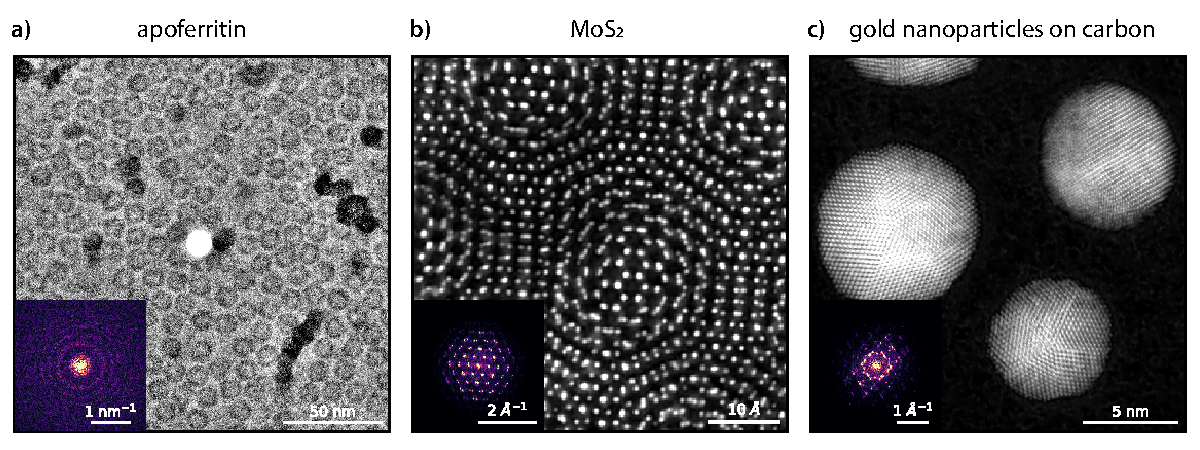
\includegraphics[width=\textwidth]{vector/iterative.pdf}
\caption{
Iterative ptychography reconstructions of
\textbf{a)} apoferritin~\cite{Berk_2024}, \textbf{b)} MoS$_2$~\cite{zhang2025atom}, and \textbf{c)} gold nanoparticles on amorphous carbon.
Aberrations coefficients were initialized using direct ptychography reconstructions in \cref{fig:exp-compare,fig:uspsample}.
}
\label{fig:iterative}
\end{figure*}

\DIFdelbegin \subsubsection{\DIFdel{Proximal-Gradient / Projection-Set Methods}}
%DIFAUXCMD
\addtocounter{subsubsection}{-1}%DIFAUXCMD
\DIFdelend \DIFaddbegin \subsubsection*{\DIFadd{Proximal-gradient / projection-set methods}}
\DIFaddend \label{sec:projection-methods}

The earliest iterative ptychographic algorithms derive from classical phase-retrieval methods in crystallography and coherent diffractive imaging~\cite{karle1985,Fienup_1982,Levi_1984,Miao_1999,Bauschke_2002,Elser_2003,Thibault_2008}.
These approaches frame reconstruction as finding an object-illumination pair $(\mathcal{O},\psi)$ lying in the intersection of two constraint sets: i) real-space constraint: the exit-wave must equal the product of the object and shifted illumination estimates, and ii) Fourier-modulus constraint: the exit-wave Fourier magnitude must match the measured intensities.

Algorithms such as \emph{error reduction} (ER)~\cite{Levi_1984}, \emph{difference map} (DM)~\cite{Elser_2003,Thibault_2008}, and \emph{relaxed averaged alternating reflections} (RAAR)~\cite{Luke_2004}, repeatedly project (and/or reflect) the exit wave between these two sets.
The canonical ER exit-wave update is given by~\cite{Bauschke_2002}:
\begin{align}
\psi_{\text{exit}}^{'(j)}(\boldsymbol{r})
&=
\mathcal{F}_{\boldsymbol{k}\to\boldsymbol{r}}^{-1}
\left\{
\frac{\sqrt{I_{\text{meas}}^{(j)}(\boldsymbol{k})}}{\left\lvert \tilde{\psi}_{\text{exit}}^{(j)}(\boldsymbol{k}) \right\rvert}
\tilde{\psi}_{\text{exit}}^{(j)}(\boldsymbol{k})
\right\}
\nonumber\\
&\equiv
\Pi_f\!\left[\psi_{\text{exit}}^{(j)}(\boldsymbol{r})\right],
\label{eq:proj-exit-wave}
\end{align}
where the Fourier-projection operator $\Pi_f$ replaces the Fourier exit-wave magnitude with the measured amplitude, retaining only its phase~\cite{Fienup_1982,Bauschke_2002}.
The object and probe updates follow from enforcing the real-space multiplicative constraint~\cite{Thibault_2008}:
\begin{align}
\mathcal{O}'(\boldsymbol{r})
&=
\frac{
\sum_j
\psi^{*}(\boldsymbol{r}-\boldsymbol{R}_j)
\psi_{\text{exit}}^{'(j)}(\boldsymbol{r})
}{
\left \lVert \psi(\boldsymbol{r}-\boldsymbol{R}_j)\right \rVert^2_{\alpha}},\\
\psi'(\boldsymbol{r})
&=
\frac{
\sum_j
\mathcal{O}^{*}(\boldsymbol{r})
\psi_{\text{exit}}^{'(j)}(\boldsymbol{r})
}{
\left \lVert\mathcal{O}(\boldsymbol{r})\right \rVert^2_{\alpha}
},
\label{eq:proj-update}
\end{align}
where $\alpha$ is a scalar 0--1 parameter controlling the maximum overlap weight in the $\lVert\cdot\rVert^2_{\alpha}$ normalization.
\begin{align}
\left \lVert\cdot \right \rVert ^2_{\alpha}
&=
(1-\alpha)\sum_j \lvert \cdot \rvert^2
+
\alpha \sum_j \lvert \cdot \rvert^2_{\text{max}}.
\label{eq:normalization}
\end{align}

DM and RAAR combine projections in more sophisticated ways to form the exit-wave update given.
In-fact, we can parametrize a family of projection-set algorithms, using the scalar parameters $(a,b,c)$:
\begin{align}
\psi_{\text{exit}}^{'(j)}(\boldsymbol{r})
&=
(1-a-b)\,\psi_{\text{exit}}^{'(j)}(\boldsymbol{r})
+
a\,\psi_{\text{exit}}^{(j)}(\boldsymbol{r})
\nonumber\\
&\quad+
b\,\Pi_f\!\left[
c\,\psi_{\text{exit}}^{(j)}(\boldsymbol{r})
+
(1-c)\,\psi_{\text{exit}}^{'(j)}(\boldsymbol{r})
\right].
\label{eq:proj-fam}
\end{align}
Named algorithms can then be recovered using specific $(a,b,c)$ combinations:
ER $(a=0,b=1,c=1)$~\cite{Levi_1984}, DM $(a=-1,b=1,c=2)$~\cite{Elser_2003}, and RAAR $(a=1-2\gamma,b=\gamma,c=2)$~\cite{Luke_2004}, with relaxation parameter $\gamma$.

Projection-set algorithms are robust and computationally simple, relying only on pointwise operations.
However, their relation to an explicit optimization problem is indirect, making them harder to generalize and sometimes slow to converge in low-redundancy or strong-scattering regimes~\cite{Varnavides_2023}.

\DIFdelbegin \subsubsection{\DIFdel{Gradient-Based Methods}}
%DIFAUXCMD
\addtocounter{subsubsection}{-1}%DIFAUXCMD
\DIFdelend \DIFaddbegin \subsubsection*{\DIFadd{Gradient-based methods}}
\DIFaddend 

A more modern view formulates ptychography as minimizing a data-fidelity loss.
For the amplitude-based noise model, the loss for a given exit wave is:
\begin{align}
\mathcal{L}
=
\sum_j
\left\lVert
\left\lvert
\tilde{\psi}_{\text{exit}}^{(j)}(\boldsymbol{k})
\right\rvert
-
\sqrt{I_{\text{meas}}^{(j)}(\boldsymbol{k})}
\right\rVert^2.
\label{eq:loss}
\end{align}

One of the earliest gradient-based ptychographic algorithms is the \emph{extended ptychographic iterative engine} (ePIE)~\cite{Maiden_2009}, which performs block-wise stochastic gradient descent (SGD) in which each scan position provides a local loss and gradient update.
Modern approaches generalize this to true mini-batch optimization methods such as SGD and Adam~\cite{Lee_2025,Gilgenbach_2025,McCray_2025}.

The amplitude loss in \cref{eq:loss}, corresponds to the \emph{maximum a posteriori} estimator under Gaussian detector noise with unit variance~\cite{Gilgenbach_2025}.
Although electron detection is fundamentally Poissonian, at moderate electron counts the \DIFdelbegin \DIFdel{Gaussian approximation becomes valid, matching the same assumption }\DIFdelend \DIFaddbegin \DIFadd{shot noise can be approximated as Gaussian with variance proportional to the mean intensity. 
After normalization by this variance, the noise becomes unit-variance and independent of probe position, yielding the same linear SNR scaling with electron dose derived for Poisson statistics in Refs. \mbox{%DIFAUXCMD
\citenum{Seki_2018,Ooe_2021} }\hskip0pt%DIFAUXCMD
and }\DIFaddend used in the WPOA noise model \cref{eq:noise-model}.

Under this approximation, the exit-wave gradient has a closed-form expression, identical to the ER Fourier-magnitude projection:
\begin{align}
\Delta \psi_{\text{exit}}^{(j)}(\boldsymbol{r})
=
\Pi_f\!\left[
\psi_{\text{exit}}^{(j)}(\boldsymbol{r})
\right]
-
\psi_{\text{exit}}^{(j)}(\boldsymbol{r}).
\label{eq:gd}
\end{align}

This can be used to update the object and illumination estimates using a form very similar to \cref{eq:proj-update}:
\begin{align}
\mathcal{O}^{' }(\boldsymbol{r})
&=
\mathcal{O}(\boldsymbol{r})
+
\beta
\frac{
\sum_j^J
\psi^{*}(\boldsymbol{r}-\boldsymbol{R}_j)
\Delta \psi_{\text{exit}}^{(j)}(\boldsymbol{r})
}{
\left\lVert
\psi(\boldsymbol{r}-\boldsymbol{R}_j)
\right\rVert^2_{\alpha}
},\\
\psi^{' }(\boldsymbol{r})
&=
\psi(\boldsymbol{r})
+
\beta
\frac{
\sum_j^J
\mathcal{O}^{*}(\boldsymbol{r})
\Delta \psi_{\text{exit}}^{(j)}(\boldsymbol{r})
}{
\left\lVert
\mathcal{O}(\boldsymbol{r})
\right\rVert^2_{\alpha}
}.
\label{eq:sgd-update}
\end{align}

Gradient-based methods offer clear statistical interpretability, support batching and adaptive learning rates, and integrate naturally with extensions such as multislice, mixed-state, and parametric probe models.
Unlike projection-set methods, they make the optimization landscape explicit, enabling principled regularization and convergence diagnostics.

\cref{fig:iterative} illustrates the advantages of iterative phase retrieval over direct methods across several experimental datasets spanning different materials classes, using the aberration coefficients optimized in \cref{fig:exp-compare}.
In \DIFdelbegin \DIFdel{each case}\DIFdelend \DIFaddbegin \DIFadd{all cases}\DIFaddend , iterative ptychography yields improved contrast, reduced artifacts, and more faithful recovery of structural features \DIFdelbegin \DIFdel{.
}\DIFdelend \DIFaddbegin \DIFadd{compared to the direct reconstructions shown in~\mbox{%DIFAUXCMD
\cref{fig:exp-compare,fig:uspsample}}\hskip0pt%DIFAUXCMD
.
This improvement is particularly evident in the Fourier transforms, which exhibit an extended transfer of high spatial frequencies, indicating enhanced resolution.
}\DIFaddend 

\DIFdelbegin \subsubsection{\DIFdel{Transfer of Information}}
%DIFAUXCMD
\addtocounter{subsubsection}{-1}%DIFAUXCMD
\DIFdelend \DIFaddbegin \subsubsection*{\DIFadd{Transfer of information}}
\DIFaddend 

Although iterative ptychography does not admit simple closed-form CTF/SSNR like the direct methods, several useful observations can be made~\cite{Varnavides_2025_ssnr}:

\begin{enumerate}
\item With a reasonably accurate probe guess, the first iteration update of ePIE/SGD effectively performs probe deconvolution under the WPOA, yielding a CTF similar to the SSB CTF.
\item As iterations proceed, the effective CTF fills in information, approaching unity everywhere.
\item Numerical tests reveal that the low-frequency SSNR of iterative ptychography matches SSB.
At higher frequencies, the SSNR plateaus to $\sqrt{2}/2$, consistent with recent Fisher information limits which suggest a STEM DQE ceiling of $1/2$~\cite{Dwyer_2024,Vega_2025,Varnavides_2025_ssnr}.
\end{enumerate}

Together, these observations show that although iterative ptychography can achieve super-resolution, the statistical information content is similar to direct linear methods at low spatial frequencies, with predictable saturation at intermediate frequencies.

\DIFdelbegin \subsection{\DIFdel{Beyond Single-slice Ptychography}}
%DIFAUXCMD
\addtocounter{subsection}{-1}%DIFAUXCMD
\DIFdelend \DIFaddbegin \subsection*{\DIFadd{Beyond single-slice ptychography}}
\DIFaddend \label{sec:beyond-ss}

The flexibility of iterative ptychography becomes especially powerful once we move beyond the single-slice, single-probe approximation used in the earlier sections.
Real experiments often deviate from this idealization: illumination is never perfectly coherent, specimens may be tens to hundreds of nanometers thick, and additional physical channels such as magnetization and inelastic excitations contribute to the detected intensity.
Iterative methods can incorporate these complexities directly into the forward model, allowing reconstructions that remain accurate well outside the WPOA regime.

As these models grow in complexity, the reconstruction problem becomes more ill-posed necessitating robust regularization.
Classical regularizers stabilize the solution by encouraging smoothness, sparsity, physical consistency, or low-rank structure~\cite{Varnavides_2023}.
Machine-learning approaches replace such hand-designed priors with learned generative models or implicit architectural biases, often yielding cleaner and more robust reconstructions, requiring less hyperparameter tuning~\cite{McCray_2025}.

In practice, high-resolution reconstructions of many materials systems almost always rely on some combination of multislice propagation, mixed-state probe modeling, and regularization.
These ingredients are essential for moving beyond the WPOA and unlocking the full information content of modern 4D-STEM experiments.

\DIFdelbegin \subsubsection{\DIFdel{Partial Coherence}}
%DIFAUXCMD
\addtocounter{subsubsection}{-1}%DIFAUXCMD
\DIFdelend \DIFaddbegin \subsubsection*{\DIFadd{Partial coherence}}
\DIFaddend 

The first major generalization is using a mixed-state illumination~\cite{Thibault_2013,Chen_2020}, which relaxes the assumption of a single, fully coherent probe.
Instead, the illumination intensity is modeled as an incoherent mixture of mutually-orthogonal probes~\cite{Odstrcil_2016}:
\begin{align}
\psi_{\text{exit}}^{(j,l)}(\boldsymbol{r})
&=
\mathcal{O}(\boldsymbol{r})
\psi^{(l)}(\boldsymbol{r}-\boldsymbol{R}_j),\\
I_{\text{model}}^{(j)}(\boldsymbol{k})
&=
\sum_l
\left\lvert
\mathcal{F}_{\boldsymbol{r}\to\boldsymbol{k}}
\left\{
\psi_{\text{exit}}^{(j,l)}(\boldsymbol{r})
\right\}
\right\rvert^2.
\label{eq:mixed-state}
\end{align}

The formalism naturally models partial spatial and temporal coherence of the electron source, including energy spread and finite source size.
In the reconstruction loop, mixed-state ptychography jointly updates the object and all probe modes so that their incoherent sum matches the measured intensity according to \cref{eq:mixed-state}.

The expressiveness of \cref{eq:mixed-state} comes at the risk of overfitting unphysical probes, necessitating strong regularization.
Conventional approaches impose orthogonality, sparsity, or low-rank constraints on the probe modes~\cite{Odstrcil_2016,Varnavides_2023}, whereas machine-learning-based reconstructions require fewer hard constraints due to their implicit regularization~\cite{McCray_2025}.

\DIFdelbegin \subsubsection{\DIFdel{Depth Information}}
%DIFAUXCMD
\addtocounter{subsubsection}{-1}%DIFAUXCMD
\DIFdelend \DIFaddbegin \subsubsection*{\DIFadd{Depth information}}
\DIFaddend 

A second often-necessary extension is the multislice approximation, which models strong multiple scattering in thicker specimens using \cref{eq:ms}.
Specifically, the modeled intensities for $N$ slices are given by:
\begin{align}
\psi_{\text{exit}}^{(j,n)}(\boldsymbol{r})
&=
\mathcal{O}^{(n)}(\boldsymbol{r})
\psi^{(n)}(\boldsymbol{r}-\boldsymbol{R}_j),
\label{eq:multi-slice-01}
\end{align}
\begin{align}
\psi^{(n)}(\boldsymbol{r})
&=
\operatorname{Prop}_{\Delta z}
\left[
\psi^{(n-1)}(\boldsymbol{r})
\right]
\quad \text{for } n \geq 2,\\
I_{\text{model}}^{(j)}(\boldsymbol{k})
&=
\left\lvert
\mathcal{F}_{\boldsymbol{r}\to\boldsymbol{k}}
\left\{
\psi_{\text{exit}}^{(j,N)}(\boldsymbol{r})
\right\}
\right\rvert^2.
\label{eq:multi-slice-02}
\end{align}

Multislice ptychography is crucial for quantitative imaging of materials far outside the weak-scattering regime, including thick crystals, buried interfaces, and defect structures~\cite{Ribet_2024}.
By explicitly modeling dynamical diffraction, the multislice framework mitigates systematic errors that appear when single-slice reconstructions attempt to explain multiple scattering using only a 2D projected potential.

As with mixed-state ptychography, this increased expressive power introduces additional degrees of freedom.
Explicit regularization along the beam direction helps stabilize the reconstruction, with machine-learning-based approaches relying on the implicit regularization of the network architecture~\cite{McCray_2025}.

Combining ptychography with tomography can substantially improve multislice depth resolution~\cite{chen2024imaging,allars2025depth}.
Approaches such as few-tilt acquisitions and joint ptychography-tomography optimization recover complementary angular information, reducing the ambiguities inherent to purely depth-slicing multislice reconstructions~\cite{Lee_2023,You_2024,Dong_2025}.
These methods achieve accurate 3D reconstructions and mitigate slice-mixing artifacts, particularly in thick or compositionally heterogeneous specimens.

\DIFdelbegin \section{\DIFdel{Outlook}}
%DIFAUXCMD
\addtocounter{section}{-1}%DIFAUXCMD
\DIFdelend \DIFaddbegin \section*{\DIFadd{Outlook and conclusions}}
\DIFaddend 

\DIFdelbegin \DIFdel{The ability of phase-retrieval techniques to recover weak scattering signals makes the approaches described here broadly applicable across materials science and engineering.
They are particularly well suited for }\DIFdelend \DIFaddbegin \DIFadd{Phase-retrieval techniques in STEM provide a unified framework for recovering specimen phase and overcoming the intrinsic contrast limitations imposed by the phase problem.
Within this framework, reconstruction fidelity is governed by the interplay between illumination diversity, sampling, and experimental geometry, which together determine the transfer of phase information.
These methods are broadly applicable to }\DIFaddend beam-sensitive \DIFdelbegin \DIFdel{, }\DIFdelend \DIFaddbegin \DIFadd{and }\DIFaddend low-atomic-number \DIFdelbegin \DIFdel{specimens such as polymers~\mbox{%DIFAUXCMD
\cite{bardot2025mechanically}}\hskip0pt%DIFAUXCMD
, biological structures}\DIFdelend \DIFaddbegin \DIFadd{materials, including biological systems}\DIFaddend ~\cite{Berk_2024,Yu_2025,Spoth_2017}, \DIFdelbegin \DIFdel{and hard–soft composites including metal–organic frameworks~\mbox{%DIFAUXCMD
\cite{Ma_2025,shen2020imaging} }\hskip0pt%DIFAUXCMD
and DNA origami~\mbox{%DIFAUXCMD
\cite{ding2022three}}\hskip0pt%DIFAUXCMD
.
Phase retrieval methods are also increasingly applied }\DIFdelend \DIFaddbegin \DIFadd{polymers~\mbox{%DIFAUXCMD
\cite{bardot2025mechanically}}\hskip0pt%DIFAUXCMD
, and hybrid structures~\mbox{%DIFAUXCMD
\cite{Li_2025,Ma_2025,shen2020imaging,ding2022three}}\hskip0pt%DIFAUXCMD
, as well as }\DIFaddend to inorganic materials \DIFdelbegin \DIFdel{, where they enable sensitivity to subtle structural variations of light elements in functional systems relevant to energy and quantum science}\DIFdelend \DIFaddbegin \DIFadd{where sensitivity to light elements is critical}\DIFaddend ~\cite{lozano2018low,kp2025electron}.
\DIFdelbegin \DIFdel{Common specimens include nanoparticles~\mbox{%DIFAUXCMD
\cite{shi2025electron,Ribet_2024,Varnavides_2023}}\hskip0pt%DIFAUXCMD
, one-dimensional nanostructures such as nanotubes~\mbox{%DIFAUXCMD
\cite{yang2016simultaneous,pelz2023solving}}\hskip0pt%DIFAUXCMD
, two-dimensional materials~\mbox{%DIFAUXCMD
\cite{jiang2018electron,o2022increasing,Susi_2025,byrne2025fabrication,zhang2025atom}}\hskip0pt%DIFAUXCMD
, thin films~\mbox{%DIFAUXCMD
\cite{dong2025sub}}\hskip0pt%DIFAUXCMD
, and cross-sectional views of thicker crystalline samples~\mbox{%DIFAUXCMD
\cite{scheid2025atomic,chen2024imaging}}\hskip0pt%DIFAUXCMD
.
}\DIFdelend 

\DIFaddbegin \DIFadd{In practice, achieving reliable phase retrieval depends sensitively on experimental conditions.
Adequate reciprocal-space overlap, accurate knowledge of aberrations (particularly defocus), and sufficient electron dose are all essential for stable inversion.
}\DIFaddend Recent work has demonstrated that ptychographic phase retrieval can \DIFdelbegin \DIFdel{even be performed }\DIFdelend \DIFaddbegin \DIFadd{be performed even }\DIFaddend on uncorrected instruments~\cite{nguyen2024achieving}, including at low accelerating voltages and small convergence angles~\cite{blackburn2025sub}.
Nevertheless, \DIFdelbegin \DIFdel{successful phase retrieval remains experimentally demanding, and in practice most samples benefit substantially }\DIFdelend \DIFaddbegin \DIFadd{most applications continue to benefit }\DIFaddend from aberration correction \DIFdelbegin \DIFdel{.
Adequate overlap in reciprocal space is essential to ensure a unique and accurate reconstruction, and phase retrieval workflows in materials science still largely rely on advanced hardware, including }\DIFdelend \DIFaddbegin \DIFadd{and advanced instrumentation, and practical workflows still rely heavily on }\DIFaddend fast pixelated detectors and \DIFdelbegin \DIFdel{aberration-correction}\DIFdelend \DIFaddbegin \DIFadd{carefully optimized acquisition parameters}\DIFaddend .

\DIFdelbegin \DIFdel{As discussed for both direct and iterative approaches, defocused acquisitions can improve information transfer in phase retrieval experiments.
However, selecting suitable experimental parameters remains challenging: reliable convergence depends sensitively on }\DIFdelend \DIFaddbegin \DIFadd{These considerations highlight several important limitations and open challenges.
Most direct phase-retrieval methods rely on linear imaging models and are therefore fundamentally limited for thick or strongly scattering specimens.
While iterative and multislice approaches can partially overcome these limitations, they introduce substantial computational cost and are not yet uniformly robust across all sample classes.
At the same time, experimental parameter selection, including }\DIFaddend defocus, probe size, and scan \DIFdelbegin \DIFdel{step, while accurate estimation of the applied defocus can be nontrivial , especially for thick specimens.
Estimating the defocus value applied during an experiment can be challenging, especially for thicker samples.
These challenges are exacerbated in very }\DIFdelend \DIFaddbegin \DIFadd{sampling, remains a critical and nontrivial aspect of successful reconstruction, particularly under }\DIFaddend low-dose \DIFdelbegin \DIFdel{experiments, where data may need to be acquired blindly and image quality assessed only through post-processing}\DIFdelend \DIFaddbegin \DIFadd{conditions where noise and incomplete sampling can lead to instability or non-uniqueness}\DIFaddend .

\DIFdelbegin \DIFdel{Direct reconstruction techniques are computationally efficient and can often be performed live }\DIFdelend \DIFaddbegin \DIFadd{From a practical perspective, direct reconstruction techniques offer a complementary advantage in computational efficiency, enabling live reconstruction }\DIFaddend during data acquisition using modern hardware~\cite{Yu_2022,Ooe_2021,Pelz_2022,Strauch_2021}.
Such \DIFdelbegin \DIFdel{on-the-fly reconstructions are }\DIFdelend \DIFaddbegin \DIFadd{real-time feedback is }\DIFaddend valuable for optimizing \DIFdelbegin \DIFdel{experimental parameters, verifying }\DIFdelend \DIFaddbegin \DIFadd{imaging conditions, assessing }\DIFaddend sample thickness, and \DIFdelbegin \DIFdel{detecting beam damagein real time}\DIFdelend \DIFaddbegin \DIFadd{monitoring beam damage}\DIFaddend .
In typical workflows, \DIFdelbegin \DIFdel{direct phase retrieval is }\DIFdelend \DIFaddbegin \DIFadd{these fast direct methods are }\DIFaddend used during acquisition, while more \DIFdelbegin \DIFdel{computationally intensive iterative reconstructions, especially those involving multislice propagation }\DIFdelend \DIFaddbegin \DIFadd{complete iterative reconstructions—especially those incorporating multislice }\DIFaddend or mixed-state \DIFdelbegin \DIFdel{modeling, are carried out }\DIFdelend \DIFaddbegin \DIFadd{models—are performed }\DIFaddend offline on GPU-equipped \DIFdelbegin \DIFdel{workstations and high-performance computer clusters}\DIFdelend \DIFaddbegin \DIFadd{systems}\DIFaddend .

Looking forward, \DIFdelbegin \DIFdel{key challenges include extending }\DIFdelend \DIFaddbegin \DIFadd{further progress will depend on addressing these limitations in a systematic way.
Improved strategies for parameter estimation and experimental design, potentially incorporating real-time feedback or adaptive acquisition, could significantly enhance robustness.
Extending }\DIFaddend phase retrieval to thicker \DIFdelbegin \DIFdel{specimens, }\DIFdelend \DIFaddbegin \DIFadd{and more strongly scattering specimens will require tighter integration of multislice forward models with efficient inversion schemes.
Finally, scaling these approaches to }\DIFaddend larger fields of view \DIFdelbegin \DIFdel{, }\DIFdelend and higher-dimensional \DIFdelbegin \DIFdel{datasets that combine phase retrieval with tomography , spectroscopy, or }\DIFdelend \DIFaddbegin \DIFadd{modalities—including tomography and }\DIFaddend time-resolved measurements\DIFdelbegin \DIFdel{, as well as adapting these methods to an increasingly diverse range of microscope configurations.
Many groups are already pushing to extend these techniques through both hardware and software advances, which will allow for more advanced materials characterization in the near future}\DIFdelend \DIFaddbegin \DIFadd{—remains a key challenge for both algorithm development and instrumentation}\DIFaddend .

\section*{Funding}

Work at the Molecular Foundry was supported by the Office of Science, Office of Basic Energy Sciences, of the U.S.\ Department of Energy under Contract No.\ DE-AC02-05CH11231.

\section*{Conflict of \DIFdelbegin \DIFdel{Interest}\DIFdelend \DIFaddbegin \DIFadd{interest}\DIFaddend }

The authors declare there are no conflicts of interest.

\section*{Author \DIFdelbegin \DIFdel{Contributions}\DIFdelend \DIFaddbegin \DIFadd{contributions}\DIFaddend }

Georgios Varnavides and Stephanie M. Ribet contributed to the article conception and design.
Georgios Varnavides implemented the linear phase estimators, and produced all simulated results.
Stephanie M. Ribet collected experimental defocused gold nanoparticle dataset and performed all experimental reconstructions.
Willem P.M. de Kleijne performed the literature review and verified the math derivations.
The first draft of the manuscript was written by Georgios Varnavides and all authors commented on previous versions of the manuscript.
All authors read and approved the final manuscript.

\section*{Data availability}

The calibrated experimental datasets supporting the findings of this study are publicly available at \url{https://doi.org/10.5281/zenodo.18449975}.
All reconstruction and analysis notebooks used to generate the figures are available at \url{https://github.com/curiousbeams/mrs-bulletin-phase-retrieval-abcs}.

\bibliography{references}

\end{document}
